\documentclass[runningheads]{llncs}

\usepackage[T1]{fontenc}
\usepackage{graphicx}
%\usepackage{color}
%\renewcommand\UrlFont{\color{blue}\rmfamily}

\usepackage{amsmath,amssymb,amsfonts}
\usepackage[inline, shortlabels]{enumitem}
\usepackage{tabularx}
\usepackage{caption}
\usepackage{listings}
% \usepackage{titlesec}
\usepackage[english]{babel}
\captionsetup{font=it}
\usepackage{ragged2e}
\usepackage[hyphens]{url}
\usepackage{hyperref}
\usepackage{xurl}
\usepackage{pifont}
\usepackage{footmisc}
\usepackage{multirow}
\usepackage{enumitem}
\usepackage{algorithm2e}
\usepackage{float}
\usepackage{listings}
\usepackage{xcolor}

\definecolor{codegreen}{rgb}{0,0.6,0}
\definecolor{codegray}{rgb}{0.5,0.5,0.5}
\definecolor{codepurple}{rgb}{0.58,0,0.82}
\definecolor{backcolour}{rgb}{0.95,0.95,0.92}
 
\lstdefinestyle{mystyle}{
    backgroundcolor=\color{backcolour},   
    commentstyle=\color{codegreen},
    keywordstyle=\color{magenta},
    numberstyle=\tiny\color{codegray},
    stringstyle=\color{codepurple},
    basicstyle=\footnotesize,
    breakatwhitespace=false,         
    breaklines=true,                 
    captionpos=b,                    
    keepspaces=true,                 
    numbers=left,                    
    numbersep=5pt,                  
    showspaces=false,                
    showstringspaces=false,
    showtabs=false,                  
    tabsize=2
}
 
\lstset{style=mystyle}

% --- Tickz
\usepackage{physics}
\usepackage{amsmath}
\usepackage{tikz}
\usepackage{mathdots}
\usepackage{yhmath}
\usepackage{cancel}
\usepackage{color}
\usepackage{siunitx}
\usepackage{array}
\usepackage{multirow}
\usepackage{amssymb}
\usepackage{gensymb}
\usepackage{tabularx}
\usepackage{extarrows}
\usepackage{booktabs}
\usetikzlibrary{fadings}
\usetikzlibrary{patterns}
\usetikzlibrary{shadows.blur}
\usetikzlibrary{shapes}

% ---------
% \usepackage{titlesec}
\usepackage{pdfpages}
\usepackage{booktabs}
\usepackage{csquotes}
\usepackage{lipsum}  
\usepackage{arydshln}
\usepackage{smartdiagram}
\usepackage[inkscapeformat=png]{svg}
\usepackage{textcomp}
\usepackage{tabularray}\UseTblrLibrary{varwidth}
\usepackage{xcolor}
\def\BibTeX{{\rm B\kern-.05em{\sc i\kern-.025em b}\kern-.08em
    T\kern-.1667em\lower.7ex\hbox{E}\kern-.125emX}}
\usepackage{cite}
\usepackage{amsmath}
\newcommand{\probP}{\text{I\kern-0.15em P}}
\usepackage{etoolbox}
\patchcmd{\thebibliography}{\section*{\refname}}{}{}{}

\setlength\tabcolsep{0.5pt}

% \renewcommand{\arraystretch}{1.7}

% \setlength{\extrarowheight}{2.5pt}
% \renewcommand{\arraystretch}{0.2}
% \renewcommand{\arraystretch}{1.7}

% --------------
% \titleclass{\subsubsubsection}{straight}[\subsection]

% \newcounter{subsubsubsection}[subsubsection]
% \renewcommand\thesubsubsubsection{\thesubsubsection.\arabic{subsubsubsection}}
% \renewcommand\theparagraph{\thesubsubsubsection.\arabic{paragraph}} % optional; useful if paragraphs are to be numbered

% \titleformat{\subsubsubsection}
%   {\normalfont\normalsize\bfseries}{\thesubsubsubsection}{1em}{}
% \titlespacing*{\subsubsubsection}
% {0pt}{3.25ex plus 1ex minus .2ex}{1.5ex plus .2ex}

% \makeatletter
% \renewcommand\paragraph{\@startsection{paragraph}{5}{\z@}%
%   {3.25ex \@plus1ex \@minus.2ex}%
%   {-1em}%
%   {\normalfont\normalsize\bfseries}}
% \renewcommand\subparagraph{\@startsection{subparagraph}{6}{\parindent}%
%   {3.25ex \@plus1ex \@minus .2ex}%
%   {-1em}%
%   {\normalfont\normalsize\bfseries}}
% \def\toclevel@subsubsubsection{4}
% \def\toclevel@paragraph{5}
% \def\toclevel@paragraph{6}
% \def\l@subsubsubsection{\@dottedtocline{4}{7em}{4em}}
% \def\l@paragraph{\@dottedtocline{5}{10em}{5em}}
% \def\l@subparagraph{\@dottedtocline{6}{14em}{6em}}
% \makeatother

% \setcounter{secnumdepth}{4}
% \setcounter{tocdepth}{4}
% --------------

\newcommand{\before}[1]{\textcolor{red}{#1}}
\newcommand{\after}[1]{\textcolor{green}{#1}}

\newcommand{\old}[1]{\textcolor{orange}{#1}}
\newcommand{\rem}[1]{\textcolor{red}{#1}}
\newcommand{\todo}[1]{\textcolor{orange}{\newline \textit{\textbf{TODO:} #1}} \newline \newline }



\newcounter{relation}
\setcounter{relation}{0}
\renewcommand{\therelation}{\arabic{relation}}
\newcommand{\relationautorefname}{Relation}

\newenvironment{relation}[1][]{%
    \refstepcounter{relation}%
    \noindent \raggedright \textit{\textbf{Relation. \therelation}} \hfill$}
{%
$ \hfill \phantom{x}

}

\newcounter{proof}
\setcounter{proof}{0}
\renewcommand{\theproof}{\arabic{proof}}
\newcommand{\proofautorefname}{Proof}

\renewenvironment{proof}[1][]{
    \refstepcounter{proof}
    \noindent \raggedright \textit{\textbf{Proof. \theproof}}

    \setlength{\leftskip}{1em}

}
{

\
\setlength{\leftskip}{0pt}
}

% --------------------------------
%             DOCUMENT
% --------------------------------

\begin{document}
\title{A MARL-based Approach for Easing MAS Organization Engineering}
%
%\titlerunning{Abbreviated paper title}
% If the paper title is too long for the running head, you can set
% an abbreviated paper title here
%
% \author{Julien Soulé\inst{1}\orcidID{0000-1111-2222-3333} \and
% Jean-Paul Jamont\inst{1}\orcidID{1111-2222-3333-4444} \and
% Michel Occello\inst{1}\orcidID{2222--3333-4444-5555} \and
% Louis-Marie Traonouez\inst{2}\orcidID{2222--3333-4444-5555} \and
% Paul Théron\inst{3}\orcidID{2222--3333-4444-5555}}
\author{Julien Soulé\inst{1} \and
Jean-Paul Jamont\inst{1} \and
Michel Occello\inst{1} \and
Louis-Marie Traonouez\inst{2} \and
Paul Théron\inst{3}}
%
\authorrunning{J. Soulé et al.}
% First names are abbreviated in the running head.
% If there are more than two authors, 'et al.' is used.
%
\institute{Univ. Grenoble Alpes, Grenoble INP, LCIS, 26000, Valence, France
    \email{\{julien.soule, jean-paul.jamont, michel.occello\}@lcis.grenoble-inp.fr}
    \and
    Thales Land and Air Systems, BL IAS, Rennes, France
    \email{louis-marie.traonouez@thalesgroup.com}
    \and
    AICA IWG, La Guillermie, France \\
    \email{paul.theron@orange.fr}
}


\maketitle              % typeset the header of the contribution

% MAS have been succefully
% For many MAS, the organization has become a critical success factor. 
% Several related methods exist to design MAS. 
% However, these methods are ...
% To enhance the quality and effectiveness of ... this paper presents an assisted approach for MAS Organization Engineering (AMOEA). 
% AMOEA guides the designer of...
% 1 phrase par contrib/key point

\begin{abstract}

    % context
    Multi-Agent Systems (MAS) have been successfully applied in industry for their ability to address complex, distributed problems, especially in IoT-based systems.
    Their efficiency in achieving given objectives and meeting design requirements is strongly dependent on the MAS organization during the engineering process of an application-specific MAS. To design a MAS that can achieve given goals, available methods rely on the designer's knowledge of the deployment environment.
    % Yet, in some cases, the deployment environment is not easily readable or handleable due to the complexity and may lead to unexpected emergent phenomena raising safety concerns.
    However, high complexity and low readability in some deployment environments make the application of these methods to be costly or raise safety concerns.
    % That stresses out the need for methodological works for assisted MAS design that could be addressed with collective AI techniques.
    % hypothesis / contribution
    In order to ease the MAS organization design regarding those concerns, we introduce an original Assisted MAS Organization Engineering Approach (AOMEA). AOMEA relies on combining a Multi-Agent Reinforcement Learning (MARL) process with an organizational model to suggest relevant organizational specifications to help in MAS engineering.
    % We introduce , an novel design approach to assist the MAS design whose underlying idea is to use Multi-Agent Reinforcement Learning with organizational specifications for both understanding and constraining the training process regarding design constraints.
    % results
    % We applied our approach in cooperative Atari games and a Cyberdefense drone swarm scenario of the 3rd CAGE Challenge. Obtained specifications are indeed consistent with design constraints and provide insights of relevant collective strategies that led to develop an explainable MAS with scores close to finalists' ones.

    \keywords{Multi-Agent Systems \and Design \and Assisted engineering}
\end{abstract}

\section{Introduction}

% Context:

MAS have drawn significant interest in the industrial field due to their ability to address complex, distributed problems~\cite{Raileanu2023}.
That paradigm enables decomposing a complex task into missions that are delegated to autonomous agents that achieve them through cooperation mechanisms. Most notably, they provide models and approaches to handle conflicting goals, parallel computation, system robustness, and scalability.
%The applications of MAS are diverse, including collective robotics, Vehicular Ad Hoc Network (VANET)\cite{Oliveira1999, Gembarski2020}.
In MAS, the organization is a fundamental concept that has an impact on how agents coordinate their activities to collaboratively achieve a common goal~\cite{Hubner2007}.
Organizational aspects address the challenge of MAS design in dynamic and uncertain environments, where runtime behavior needs to be flexible~\cite{Kathleen2020}. Organization in MAS design is a central concept in methodologies and frameworks enabling the engineering of application-specific MAS~\cite{Bakliwal2018}.

MAS design/development methods have often been proposed jointly with organizational models to help designers find suitable organizational specifications enabling a MAS to reach a goal efficiently. Methods such as GAIA~\cite{Wooldridge2000,Cernuzzi2014}, ADELFE~\cite{Mefteh2015}, or DIAMOND~\cite{Jamont2015}, KB-ORG~\cite{Sims2008} provide protocols that rely on the designer's experience to hand-craft the agent's rules (also called \textbf{policies}) leveraging \textbf{self/re-organization} mechanisms to adapt the MAS on the deployment environment.
These aforementioned methods are commonly applied through simulations for they enable a safe monitoring framework for the design process and assessment. A MAS developed in simulated environments with high fidelity to the target system is expected to be transferred to the target system to perform adequately~\cite{Schon2021}.

The designer defines the agents' policies in various ways ranging from the agent's individual point of view to the global organization point of view. A properly designed MAS is expected to show emerging or chosen organizations enabling reaching a goal~\cite{Picard2009}. That design approach often takes place as an iterative process proceeding by trial and error. Yet, it shows the following limitations:
\begin{enumerate*}[label=\roman*),itemjoin={;\quad}]
    \item It requires sufficiently experienced designers
    \item It may be costly to converge towards a sufficiently estimated successful MAS
    \item It gets difficult to apply for complex and highly dimensional target deployment environments.
\end{enumerate*}
For instance, research in Autonomous Intelligent Cyberdefense Agents~\cite{Kott2023} (AICA) aims to develop cooperative Cyberdefense agents deployed in highly complex computer networks. The development of an AICA faces the lack of visual and intuitive comprehension of the networked environments such as company networks.

% Problem:

Even though some methods may automate some parts of the MAS organization design such as KB-ORG~\cite{Sims2008}, they still require some knowledge and manual interactions to guide the designing process. Indeed, there is a need for
\begin{enumerate*}[label=\roman*),itemjoin={; and \ }]
    \item Finding automatically suited agents' policies satisfying design constraints
    \item Making explicit the organizational mechanisms that emerge from trained agents for the design process.
\end{enumerate*}

% Contribution

To address these issues, we introduce AMOEA, a MAS design approach whose underlying idea is to link a given MARL process with an organizational model that links the on-training agents' policies with explicit organizational specifications. It can be viewed as a tool for engineering to automatically generate relevant exploitable organizational specifications only regarding the performance in achieving the given goal and the design constraints. For the designer, the obtained organizational specifications are insights into the organizational mechanisms to set up for developing a MAS that meets performance requirements.

% Results

% We applied AOMEA in three spatial Atari games with various required degree of cooperation among agents so they achieve a goal the most efficiently; and additionally respecting organizational specifications as design constraints. Obtained organizational specifications are indeed exploitable, coherent with expectations, and respect design constraints.
%We also applied our approach, in a Cyberdefense drone swarm environment whose resulting organizational specifications led to develop a MAS with scores comparable to the leading ones.

Section II starts by introducing the theoretical background of AOMEA and focuses on the fundamental concepts we used for the organizational models and MARL.
% and the motivation for integrating a MAS organizational model into a MARL process in order to enhance the MAS design process.
In section III, we present AOMEA from the approach to the implemented tool. We assessed AOMEA in four simulated environments and discussed the obtained results in section IV. Finally, section V concludes on the AOMEA's viability and highlights limitations to overcome and future works as well.

% ====================================================================================================

\section{Theoretical background}

% // Mettre en avant les briques du raisonnement en expliquant le titre pour préparer l'introduction de la contribution avec AOMEA sans les justifier (sans faire de comparaison avec l'existant, pas d'édt, dire juste les points forts)

% Organization
%   -> moise (justifier parmi les existants)

% MAS methodologies (ALAADIN, GAIAI mais pas de moyens pour trouver une organisation automatiquemenet)

% MARL (basiques) // DECPOMDP (basiques)

In this section, we present the basics of the $\mathcal{M}OISE^+$ organizational model and the MARL basics on which our contribution is built.

\subsection{Multi-Agent Systems context}

% definition, modèle AEIO, focus Moise, Dec-POMDP

An agent is an entity immersed in an environment that perceives observation and makes a decision to act autonomously in the environment to achieve the objectives assigned to it.
Agent types include event-driven reactive to deal with uncertainties in an environment or cognitive proactive agents that leverage interactions with other agents. A MAS is a set of agents in a shared environment where each agent has only a local perception. These agents are to be endowed with self/re-organizing capabilities that allow them to adaptively modify their organizational structure according to their environment.

A MAS is strongly linked to the organization entity (we simply call \textbf{organization}) we consider it to always exist through the running agents' interactions even though it may be implicit.
%
% These methods are essential for ensuring that MAS can effectively coordinate, communicate, and execute tasks in a distributed and often dynamic environment.
% Most notable methods include
% \emph{Tropos} which is an agent-oriented software development methodology that emphasizes early requirements analysis and the continuous refinement of these requirements through the design and implementation phases~\cite{Bresciani2004};
% \emph{Gaia}, a methodology for the analysis and design of MAS, focusing on the organizational structure of the system~\cite{Zambonelli2003}; \emph{DIAMOND} which relies on a four phases iterative approach to enhance the development of multi-agent physical system; and {ADELFE} that use skills and attitudes during the design to create self-organizing systems and meet the final requirements.
% As part of methodological works, it is also worth noting the AEIO (Voyelles) model that emphasizes structuring entities within multi-agent systems by incorporating agents, environment, interactions, and organization as key components.
%
An \textbf{organizational model} specifies (at least partially) the organization whether it is used as a medium to describe an explicit known organization in a top-down way, or describing an implicit organization in a bottom-up way. An example of organizational model is the \emph{Agent/Group/Role} (AGR) model~\cite{Ferber2004}. We refer to the \textbf{organizational specifications}, the components used in an organizational model to characterize the organization. $\mathcal{M}OISE^+$ is an organizational model with which it is possible to link agents' policies to organizational specifications. It takes into account the social aspects between agents explicitly whereas \emph{AGR} focuses on the integration of standards oriented towards design. $\mathcal{M}OISE^+$~\cite{Hubner2007} considers three types of specifications:

The \textbf{structural specifications} describe the means agents can leverage to achieve a goal. It comprises the set of \emph{roles}, sub-groups, intra-group and inter-group \emph{links}, intra-group and inter-group \emph{compatibilities}, and the role and sub-group \emph{cardinalities}.
A \emph{link} indicates whether two roles are related because of acquaintance, communication, or authority ties. A \emph{compatibility} indicates whether two roles can be adopted by the same agent. Role and sub-group \emph{cardinalities} respectively refer to the minimal and maximal number of roles and sub-groups.

The \textbf{functional specifications} describe the way to achieve a goal. It comprises \emph{social schemes} and \emph{preference order}. A \emph{social scheme} is described by global goals, mission labels with plans, and the cardinality of agents committed to a mission. A \emph{preference order} means an agent has a social preference to commit to a specific mission among several possible ones.

The \textbf{deontic specifications} enable linking functional and structural specifications through a set of \emph{permissions} and obligations. A \emph{permission} means an agent playing role $\rho_a$ is permitted to commit to mission $m$ for a given time constraint $tc$. Similarly, an \emph{obligation} means an agent playing role $\rho_a$ has to commit to mission $m$ for a given time constraint $tc$. A time constraint $tc $ specifies a set of periods determining whether a permission or an obligation is valid.

% Yet, these methodological works significantly rely on human designers' experience while none of them enable automating the assistance of the MAS design process by guaranteeing sufficient efficiency while taking into account organizational aspects in a multi-agent context.

\subsection{MARL basics}

Reinforcement learning is a machine learning paradigm where agents learn to make decisions by interacting with an environment. The goal is for the agent to maximize a cumulative reward signal over time through a trial-and-error process.
MARL extends this concept to multiple agents that simultaneously learn to adapt their strategies while considering the actions and influences of other agents. That pushes agents to rely on cooperation, competition, and coordination mechanisms.

MARL enables automatically converging towards agents’ policies that enable reaching the given goal. Yet, unlike human-based design, the trained agents' logic is explicitly specified from a collective point of view. Few works attempt to address that issue and few are oriented for methodological purposes.
Kazhdan et. al.~\cite{Kazhdan2020} proposed means to extract symbolic models from MARL systems that improve the interpretability of MARL systems.
Wang et. al.~\cite{Wang2020} introduced a role-oriented MARL approach where roles are emergent, and agents with similar roles tend to share their learning and specialize in certain sub-tasks.
Tosic et. al~\cite{Tosic2010} proposed a framework for addressing coordination in collaborative MAS relying on the communication capabilities of multi-agent systems.
Zheng et. al.~\cite{Zheng2018} presented a platform for MARL that aims to facilitate research on artificial collective intelligence by providing a comprehensive set of baselines and evaluation metrics to benchmark the performance of MARL algorithms.

Markovian models are required to model the environment and apply MARL techniques. As a commonly used, Decentralized Dec-POMDP~\cite{Oliehoek2016} considers multiple agents in a similar MAS fashion. It relies on stochastic processes to model the uncertainty of the environment for the changes induced by the actions, the received observations, and the communications as well. Its reward function is common to agents which fosters training for collaborative oriented actions~\cite{Beynier2013}. Formally, a Dec-POMDP is a 7-tuple $(S,\{A_i\},T,R,\{\Omega_i\},O,\gamma)$ , where: $S = \{s_1, ..s_{|S|}\}$: The set of the possible states; $A_{i} = \{a_{1}^{i},..,a_{|A_{i}|}^{i}\}$: The set of the possible actions for agent $i$; $T$ so that $T(s,a,s') = \probP{(s'|s,a)}$ : The set of conditional transition probabilities between states; $R: S \times A \times S \rightarrow \mathbb{R}$: The reward function; $\Omega_{i} = \{o_{1}^{i},..,o_{|\Omega_{i}|}^{i}\}$: The set of observations for agent $ag_i$; $O$ so that $O(s',a,o) = \probP{(o|s',a)}$ : The set of conditional observation probabilities; $\gamma \in [0,1]$, the discount factor.

We refer to \textbf{solving} the Dec-POMDP for the team $t$ as finding a joint policy $\pi_{joint,i} \in \Pi_{joint}$ that maximizes the expected cumulative reward over a finite horizon.
We refer to \textbf{sub-optimally solving} the Dec-POMDP at $s$ expectancy as finding the joint policies $\pi_{joint,i} \in \Pi_{joint}$ that gets the expected cumulative reward over a finite horizon at least at $s \in \mathbb{R}$.

% ====
% \paragraph{\textbf{Method Fragments and Model Transformations}}
% A set of method fragments for developing MAS, which is grounded on the development process of two multi-agent systems, emphasizes the importance of model transformations in the engineering process~\cite{Garcia2011}. These fragments can be seen as modular methodologies that can be adapted and reused across different MAS projects, providing a flexible approach to system development.

% \paragraph{\textbf{Meta-Models for Analysis and Design}}
% The use of meta-models is reported to improve analysis and design activities in MAS engineering~\cite{Gomez2004}. Meta-models provide a high-level abstraction that can help in understanding and designing the complex interactions and behaviors of agents within the system, facilitating a more structured approach to MAS development.

% \paragraph{\textbf{Agent-Oriented Software Engineering Paradigms}}

% Agent technology represents a new software engineering paradigm that offers fresh prospects for analyzing, designing, and building software systems~\cite{Li2016}. This paradigm shift towards agent-oriented software engineering (AOSE) encourages developers to think in terms of autonomous agents and their interactions, leading to more robust and adaptable MAS.

% \paragraph{\textbf{Comprehensive Methodologies}}

% \paragraph{\textbf{Characterization of emergent collective strategies}}

% % Collective explainable AI: Explaining cooperative strategies and agent contribution in multiagent reinforcement learning with shapley values
% Heuillet et. al.~\cite{Heuillet2022} proposes a novel approach to explain cooperative strategies in multiagent reinforcement learning (RL) using Shapley values, a game theory concept used in eXplainable AI (XAI). The study aims to make deep RL more comprehensible and address the need for methods that provide better understanding and interpretability. The experimental results on Multiagent Particle and Sequential Social Dilemmas demonstrate the effectiveness of Shapley values in explaining the rationale behind decisions taken by agents. However, the article also highlights that Shapley values can only provide general explanations about a model and cannot explain specific actions taken by agents. The authors suggest that future work should focus on addressing these limitations. The study's implications extend to areas such as non-discriminatory decision making, ethical and responsible AI-derived decisions, and policy making under fairness constraints.

% % Social Influence as Intrinsic Motivation for Multi-Agent Deep Reinforcement Learning
% Jaques et. al.~\cite{Jaques2019} proposes a mechanism for achieving coordination and communication in MARL by rewarding agents for having causal influence over other agents' actions. This causal influence is assessed using counterfactual reasoning, where agents simulate alternate actions to compute their effect on the behavior of other agents. The paper demonstrates that this approach leads to enhanced coordination and communication, as well as more meaningful learned communication protocols. The proposed method is shown to significantly increase the learning curves of the deep reinforcement learning agents, leading to more diversified team behavior and more successful performance of the population as a whole. The paper also highlights that the influence rewards for all agents can be computed in a decentralized way, opening up new opportunities for research in this area.

% \paragraph{\textbf{Adaptation of MARL to meet requirements}}

% % Efficient MARL through automated supervision
% Chongjie et. al.~\cite{Chongjie2008} proposes a unified mechanism for achieving coordination and communication in MARL. The approach involves training multiple agents to independently maximize their own individual reward without sharing weights. The paper introduces a method for automated supervision, which enables the agents to learn to coordinate and communicate effectively. This automated supervision mechanism leads to enhanced coordination, communication, and more meaningful learned communication protocols, ultimately improving the learning curves of the deep reinforcement learning agents and the overall performance of the agent population
% %
% % Self-Organized Group for Cooperative MARL
% Shao et. al.~\cite{Shao2022} introduces a method called Self-Organized Group (SOG) for cooperative MARL. In this approach, a certain number of agents are randomly elected to be conductors, and the corresponding groups are constructed with conductor-follower consensus, allowing the groups to be re-organized at regular intervals. The organized group under the unified command of a conductor is found to embed the multi-agent system with stronger zero-shot generalization ability compared to traditional methods. The SOG method provides strong adaptability to scenarios with varying numbers of agents and varying agent sight. The paper presents this approach as a mechanism to enhance cooperative multi-agent tasks with dynamic characteristics, aiming to improve the adaptability and generalization of MARL systems
%
% % A MARL model of common-pool resource appropriation
% Perolat et. al.~\cite{Perolat2017} introduces a model that focuses on common-pool resource appropriation, a multi-agent social dilemma that includes issues such as sustainable use of fresh water, common fisheries, grazing pastures, and irrigation systems. The model emphasizes the importance of trial-and-error learning in addressing the challenges of common-pool resource sustainability and inequality. It explores the emergent behavior of groups of independently learning agents in a partially observed Markov game, shedding light on the relationship between exclusion, cooperation, and sustainability in the context of resource appropriation. The research highlights the potential of deep reinforcement learning in understanding and addressing complex societal and environmental challenges related to common-pool resource management. The paper provides valuable insights into the application of MARL in the context of real-world social dilemmas and resource management
%
% Promoting Coordination through Policy Regularization in Multi-Agent Deep Reinforcement Learning
% Roy et. al.~\cite{Roy2020} addresses the challenge of inducing coordination between agents in MARL. The research investigates the use of policy regularization to promote inter-agent coordination and discusses two approaches based on inter-agent modeling and synchronized sub-policy selection. The proposed methods are designed to improve cooperative behaviors without relying on explicit communication channels, allowing agents to exhibit coordinated behaviors during testing when acting in a decentralized fashion. The paper presents two policy regularization methods, TeamReg and CoachReg, and evaluates their performance on challenging cooperative multi-agent problems, showing improved results. The research contributes to the advancement of coordination-driven multi-agent approaches in reinforcement learning and provides valuable insights into promoting inter-agent coordination through policy regularization.

% Eventually, among considered works, none are specifically using an organizational model as a general way for both expressing the MARL resulting through OCPV; and constraining the MARL itself according to organizational specifications. It appears that augmenting MARL with an organizational model so it can be core of a aided-engineering MAS design approach; is not explicitly covered as far as we know.

% ====================================================================================================

\section{AOMEA approach}

% Mettre d'abord en avant le shcéma général de l'approche
% Donner la philosophie de l'approche

% 	Global overview (Fig 1)
% 	theoreetical core
% 	Engineering
%   Implémentation (vers une implémentation de type PoC)

\subsection{Overview}

\begin{figure}[h!]
    \centering
    


\tikzset{every picture/.style={line width=0.75pt}} %set default line width to 0.75pt        

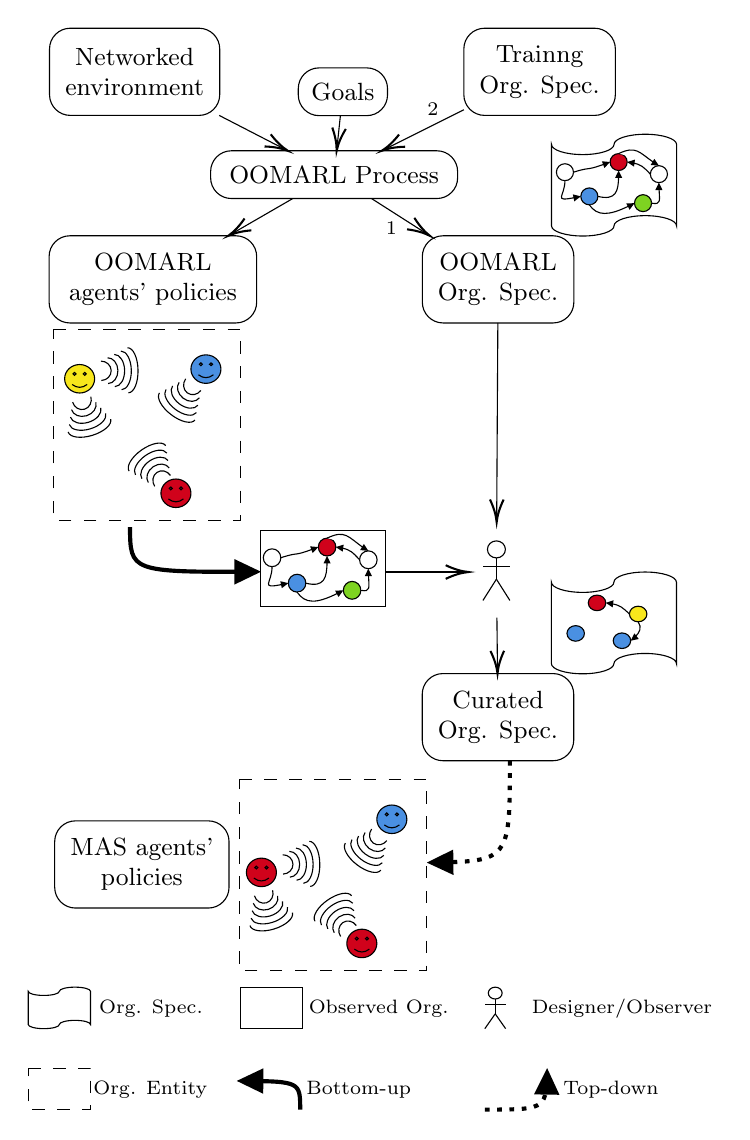
\begin{tikzpicture}[x=0.75pt,y=0.75pt,yscale=-1,xscale=1]
%uncomment if require: \path (0,567); %set diagram left start at 0, and has height of 567

%Flowchart: Punched Tape [id:dp09352793636343182] 
\draw  [fill={rgb, 255:red, 255; green, 255; blue, 255 }  ,fill opacity=1 ] (260,284.9) .. controls (260,287.61) and (266.74,289.81) .. (275.06,289.81) .. controls (283.38,289.81) and (290.12,287.61) .. (290.12,284.9) .. controls (290.12,282.2) and (296.87,280) .. (305.18,280) .. controls (313.5,280) and (320.25,282.2) .. (320.25,284.9) -- (320.25,324.13) .. controls (320.25,321.42) and (313.5,319.23) .. (305.18,319.23) .. controls (296.87,319.23) and (290.12,321.42) .. (290.12,324.13) .. controls (290.12,326.84) and (283.38,329.03) .. (275.06,329.03) .. controls (266.74,329.03) and (260,326.84) .. (260,324.13) -- cycle ;
%Shape: Ellipse [id:dp8537944349912123] 
\draw  [fill={rgb, 255:red, 208; green, 2; blue, 27 }  ,fill opacity=1 ] (277.77,294.86) .. controls (277.77,292.79) and (279.66,291.11) .. (281.98,291.11) .. controls (284.3,291.11) and (286.19,292.79) .. (286.19,294.86) .. controls (286.19,296.94) and (284.3,298.62) .. (281.98,298.62) .. controls (279.66,298.62) and (277.77,296.94) .. (277.77,294.86) -- cycle ;
%Shape: Ellipse [id:dp6897748103188357] 
\draw  [fill={rgb, 255:red, 248; green, 231; blue, 28 }  ,fill opacity=1 ] (297.6,300.23) .. controls (297.6,298.15) and (299.49,296.47) .. (301.81,296.47) .. controls (304.13,296.47) and (306.02,298.15) .. (306.02,300.23) .. controls (306.02,302.3) and (304.13,303.98) .. (301.81,303.98) .. controls (299.49,303.98) and (297.6,302.3) .. (297.6,300.23) -- cycle ;
%Shape: Ellipse [id:dp4802320082509959] 
\draw  [fill={rgb, 255:red, 74; green, 144; blue, 226 }  ,fill opacity=1 ] (289.79,313.09) .. controls (289.79,311.02) and (291.67,309.34) .. (294,309.34) .. controls (296.32,309.34) and (298.2,311.02) .. (298.2,313.09) .. controls (298.2,315.17) and (296.32,316.85) .. (294,316.85) .. controls (291.67,316.85) and (289.79,315.17) .. (289.79,313.09) -- cycle ;
%Curve Lines [id:da7546101861138359] 
\draw [fill={rgb, 255:red, 255; green, 255; blue, 255 }  ,fill opacity=1 ]   (297.6,300.23) .. controls (294.11,296.93) and (293.1,296) .. (289.08,295.29) ;
\draw [shift={(286.19,294.86)}, rotate = 7.39] [fill={rgb, 255:red, 0; green, 0; blue, 0 }  ][line width=0.08]  [draw opacity=0] (3.57,-1.72) -- (0,0) -- (3.57,1.72) -- cycle    ;
%Shape: Ellipse [id:dp693668966316707] 
\draw  [fill={rgb, 255:red, 74; green, 144; blue, 226 }  ,fill opacity=1 ] (267.5,309.58) .. controls (267.5,307.51) and (269.38,305.83) .. (271.71,305.83) .. controls (274.03,305.83) and (275.91,307.51) .. (275.91,309.58) .. controls (275.91,311.65) and (274.03,313.33) .. (271.71,313.33) .. controls (269.38,313.33) and (267.5,311.65) .. (267.5,309.58) -- cycle ;
%Curve Lines [id:da5612242217579502] 
\draw [fill={rgb, 255:red, 255; green, 255; blue, 255 }  ,fill opacity=1 ]   (301.81,303.98) .. controls (303.69,306.69) and (302.57,309.05) .. (300.45,311.16) ;
\draw [shift={(298.2,313.09)}, rotate = 322.38] [fill={rgb, 255:red, 0; green, 0; blue, 0 }  ][line width=0.08]  [draw opacity=0] (3.57,-1.72) -- (0,0) -- (3.57,1.72) -- cycle    ;

%Shape: Rectangle [id:dp7949048767988509] 
\draw  [dash pattern={on 4.5pt off 4.5pt}] (20.05,163.11) -- (110.42,163.11) -- (110.42,255.04) -- (20.05,255.04) -- cycle ;
%Shape: Smiley Face [id:dp8425156316307105] 
\draw  [fill={rgb, 255:red, 248; green, 231; blue, 28 }  ,fill opacity=1 ] (25.48,186.89) .. controls (25.48,183.1) and (28.71,180.03) .. (32.71,180.03) .. controls (36.7,180.03) and (39.94,183.1) .. (39.94,186.89) .. controls (39.94,190.68) and (36.7,193.75) .. (32.71,193.75) .. controls (28.71,193.75) and (25.48,190.68) .. (25.48,186.89) -- cycle ; \draw  [fill={rgb, 255:red, 248; green, 231; blue, 28 }  ,fill opacity=1 ] (29.53,184.56) .. controls (29.53,184.18) and (29.85,183.87) .. (30.25,183.87) .. controls (30.65,183.87) and (30.97,184.18) .. (30.97,184.56) .. controls (30.97,184.94) and (30.65,185.24) .. (30.25,185.24) .. controls (29.85,185.24) and (29.53,184.94) .. (29.53,184.56) -- cycle ; \draw  [fill={rgb, 255:red, 248; green, 231; blue, 28 }  ,fill opacity=1 ] (34.44,184.56) .. controls (34.44,184.18) and (34.77,183.87) .. (35.16,183.87) .. controls (35.56,183.87) and (35.89,184.18) .. (35.89,184.56) .. controls (35.89,184.94) and (35.56,185.24) .. (35.16,185.24) .. controls (34.77,185.24) and (34.44,184.94) .. (34.44,184.56) -- cycle ; \draw   (29.09,189.64) .. controls (31.5,191.47) and (33.91,191.47) .. (36.32,189.64) ;
%Shape: Arc [id:dp7103754459108031] 
\draw  [draw opacity=0] (47.66,206.32) .. controls (47.66,206.32) and (47.66,206.32) .. (47.66,206.32) .. controls (48.43,208.93) and (44.47,212.43) .. (38.81,214.15) .. controls (33.16,215.87) and (27.96,215.15) .. (27.19,212.54) -- (37.43,209.43) -- cycle ; \draw   (47.66,206.32) .. controls (47.66,206.32) and (47.66,206.32) .. (47.66,206.32) .. controls (48.43,208.93) and (44.47,212.43) .. (38.81,214.15) .. controls (33.16,215.87) and (27.96,215.15) .. (27.19,212.54) ;  
%Shape: Arc [id:dp9993647702991559] 
\draw  [draw opacity=0] (45.27,203.61) .. controls (46.04,206.22) and (42.73,209.53) .. (37.89,211) .. controls (33.04,212.48) and (28.49,211.55) .. (27.73,208.94) -- (36.5,206.28) -- cycle ; \draw   (45.27,203.61) .. controls (46.04,206.22) and (42.73,209.53) .. (37.89,211) .. controls (33.04,212.48) and (28.49,211.55) .. (27.73,208.94) ;  
%Shape: Arc [id:dp33021260729129986] 
\draw  [draw opacity=0] (42.88,200.9) .. controls (42.88,200.9) and (42.88,200.9) .. (42.88,200.9) .. controls (43.65,203.51) and (41,206.62) .. (36.96,207.85) .. controls (32.92,209.08) and (29.03,207.96) .. (28.26,205.35) -- (35.57,203.12) -- cycle ; \draw   (42.88,200.9) .. controls (42.88,200.9) and (42.88,200.9) .. (42.88,200.9) .. controls (43.65,203.51) and (41,206.62) .. (36.96,207.85) .. controls (32.92,209.08) and (29.03,207.96) .. (28.26,205.35) ;  
%Shape: Arc [id:dp7515950702187679] 
\draw  [draw opacity=0] (40.5,198.2) .. controls (40.5,198.2) and (40.5,198.2) .. (40.5,198.2) .. controls (40.5,198.2) and (40.5,198.2) .. (40.5,198.2) .. controls (41.26,200.81) and (39.27,203.72) .. (36.04,204.7) .. controls (32.81,205.68) and (29.57,204.36) .. (28.8,201.75) .. controls (28.8,201.75) and (28.8,201.75) .. (28.8,201.75) -- (34.65,199.97) -- cycle ; \draw   (40.5,198.2) .. controls (40.5,198.2) and (40.5,198.2) .. (40.5,198.2) .. controls (40.5,198.2) and (40.5,198.2) .. (40.5,198.2) .. controls (41.26,200.81) and (39.27,203.72) .. (36.04,204.7) .. controls (32.81,205.68) and (29.57,204.36) .. (28.8,201.75) .. controls (28.8,201.75) and (28.8,201.75) .. (28.8,201.75) ;  
%Shape: Arc [id:dp17995425823285305] 
\draw  [draw opacity=0] (38.11,195.49) .. controls (38.11,195.49) and (38.11,195.49) .. (38.11,195.49) .. controls (38.11,195.49) and (38.11,195.49) .. (38.11,195.49) .. controls (38.88,198.1) and (37.53,200.81) .. (35.11,201.55) .. controls (32.69,202.29) and (30.1,200.77) .. (29.34,198.16) -- (33.72,196.82) -- cycle ; \draw   (38.11,195.49) .. controls (38.11,195.49) and (38.11,195.49) .. (38.11,195.49) .. controls (38.11,195.49) and (38.11,195.49) .. (38.11,195.49) .. controls (38.88,198.1) and (37.53,200.81) .. (35.11,201.55) .. controls (32.69,202.29) and (30.1,200.77) .. (29.34,198.16) ;  

%Shape: Arc [id:dp8934563741256025] 
\draw  [draw opacity=0] (55.78,171.93) .. controls (58.46,171.87) and (60.73,176.69) .. (60.84,182.69) .. controls (60.96,188.7) and (58.88,193.6) .. (56.21,193.66) -- (55.99,182.79) -- cycle ; \draw   (55.78,171.93) .. controls (58.46,171.87) and (60.73,176.69) .. (60.84,182.69) .. controls (60.96,188.7) and (58.88,193.6) .. (56.21,193.66) ;  
%Shape: Arc [id:dp5963815446588989] 
\draw  [draw opacity=0] (52.58,173.54) .. controls (55.26,173.49) and (57.51,177.62) .. (57.61,182.76) .. controls (57.71,187.9) and (55.62,192.12) .. (52.94,192.17) -- (52.76,182.86) -- cycle ; \draw   (52.58,173.54) .. controls (55.26,173.49) and (57.51,177.62) .. (57.61,182.76) .. controls (57.71,187.9) and (55.62,192.12) .. (52.94,192.17) ;  
%Shape: Arc [id:dp3378668028957823] 
\draw  [draw opacity=0] (49.38,175.16) .. controls (49.38,175.16) and (49.38,175.16) .. (49.38,175.16) .. controls (49.38,175.16) and (49.38,175.16) .. (49.38,175.16) .. controls (52.06,175.11) and (54.3,178.54) .. (54.38,182.82) .. controls (54.46,187.11) and (52.36,190.63) .. (49.68,190.68) -- (49.53,182.92) -- cycle ; \draw   (49.38,175.16) .. controls (49.38,175.16) and (49.38,175.16) .. (49.38,175.16) .. controls (49.38,175.16) and (49.38,175.16) .. (49.38,175.16) .. controls (52.06,175.11) and (54.3,178.54) .. (54.38,182.82) .. controls (54.46,187.11) and (52.36,190.63) .. (49.68,190.68) ;  
%Shape: Arc [id:dp7870035207223711] 
\draw  [draw opacity=0] (46.18,176.78) .. controls (48.86,176.72) and (51.08,179.46) .. (51.15,182.89) .. controls (51.21,186.32) and (49.1,189.14) .. (46.42,189.2) -- (46.3,182.99) -- cycle ; \draw   (46.18,176.78) .. controls (48.86,176.72) and (51.08,179.46) .. (51.15,182.89) .. controls (51.21,186.32) and (49.1,189.14) .. (46.42,189.2) ;  
%Shape: Arc [id:dp7731275981870975] 
\draw  [draw opacity=0] (42.98,178.39) .. controls (42.98,178.39) and (42.98,178.39) .. (42.98,178.39) .. controls (45.65,178.34) and (47.86,180.38) .. (47.91,182.95) .. controls (47.96,185.53) and (45.83,187.65) .. (43.16,187.71) -- (43.07,183.05) -- cycle ; \draw   (42.98,178.39) .. controls (42.98,178.39) and (42.98,178.39) .. (42.98,178.39) .. controls (45.65,178.34) and (47.86,180.38) .. (47.91,182.95) .. controls (47.96,185.53) and (45.83,187.65) .. (43.16,187.71) ;  

%Shape: Smiley Face [id:dp9460068866596214] 
\draw  [fill={rgb, 255:red, 208; green, 2; blue, 27 }  ,fill opacity=1 ] (71.87,242.05) .. controls (71.87,238.26) and (75.1,235.19) .. (79.1,235.19) .. controls (83.09,235.19) and (86.33,238.26) .. (86.33,242.05) .. controls (86.33,245.84) and (83.09,248.92) .. (79.1,248.92) .. controls (75.1,248.92) and (71.87,245.84) .. (71.87,242.05) -- cycle ; \draw  [fill={rgb, 255:red, 208; green, 2; blue, 27 }  ,fill opacity=1 ] (75.91,239.72) .. controls (75.91,239.34) and (76.24,239.03) .. (76.64,239.03) .. controls (77.04,239.03) and (77.36,239.34) .. (77.36,239.72) .. controls (77.36,240.1) and (77.04,240.4) .. (76.64,240.4) .. controls (76.24,240.4) and (75.91,240.1) .. (75.91,239.72) -- cycle ; \draw  [fill={rgb, 255:red, 208; green, 2; blue, 27 }  ,fill opacity=1 ] (80.83,239.72) .. controls (80.83,239.34) and (81.15,239.03) .. (81.55,239.03) .. controls (81.95,239.03) and (82.28,239.34) .. (82.28,239.72) .. controls (82.28,240.1) and (81.95,240.4) .. (81.55,240.4) .. controls (81.15,240.4) and (80.83,240.1) .. (80.83,239.72) -- cycle ; \draw   (75.48,244.8) .. controls (77.89,246.63) and (80.3,246.63) .. (82.71,244.8) ;
%Shape: Arc [id:dp2662505393390908] 
\draw  [draw opacity=0] (56.53,231.38) .. controls (56.53,231.38) and (56.53,231.38) .. (56.53,231.38) .. controls (56.53,231.38) and (56.53,231.38) .. (56.53,231.38) .. controls (55.02,229.13) and (57.74,224.56) .. (62.6,221.17) .. controls (67.47,217.77) and (72.64,216.84) .. (74.15,219.09) -- (65.34,225.24) -- cycle ; \draw   (56.53,231.38) .. controls (56.53,231.38) and (56.53,231.38) .. (56.53,231.38) .. controls (56.53,231.38) and (56.53,231.38) .. (56.53,231.38) .. controls (55.02,229.13) and (57.74,224.56) .. (62.6,221.17) .. controls (67.47,217.77) and (72.64,216.84) .. (74.15,219.09) ;  
%Shape: Arc [id:dp5533657200850002] 
\draw  [draw opacity=0] (59.62,233.22) .. controls (59.62,233.22) and (59.62,233.22) .. (59.62,233.22) .. controls (58.11,230.97) and (60.26,226.79) .. (64.43,223.88) .. controls (68.6,220.97) and (73.21,220.43) .. (74.72,222.68) -- (67.17,227.95) -- cycle ; \draw   (59.62,233.22) .. controls (59.62,233.22) and (59.62,233.22) .. (59.62,233.22) .. controls (58.11,230.97) and (60.26,226.79) .. (64.43,223.88) .. controls (68.6,220.97) and (73.21,220.43) .. (74.72,222.68) ;  
%Shape: Arc [id:dp130720604660594] 
\draw  [draw opacity=0] (62.71,235.05) .. controls (61.19,232.8) and (62.78,229.02) .. (66.26,226.59) .. controls (69.73,224.17) and (73.78,224.02) .. (75.29,226.27) -- (69,230.66) -- cycle ; \draw   (62.71,235.05) .. controls (61.19,232.8) and (62.78,229.02) .. (66.26,226.59) .. controls (69.73,224.17) and (73.78,224.02) .. (75.29,226.27) ;  
%Shape: Arc [id:dp7777326608896638] 
\draw  [draw opacity=0] (65.79,236.88) .. controls (65.79,236.88) and (65.79,236.88) .. (65.79,236.88) .. controls (64.28,234.64) and (65.31,231.24) .. (68.09,229.3) .. controls (70.87,227.36) and (74.35,227.61) .. (75.86,229.86) -- (70.83,233.37) -- cycle ; \draw   (65.79,236.88) .. controls (65.79,236.88) and (65.79,236.88) .. (65.79,236.88) .. controls (64.28,234.64) and (65.31,231.24) .. (68.09,229.3) .. controls (70.87,227.36) and (74.35,227.61) .. (75.86,229.86) ;  
%Shape: Arc [id:dp4348101062357661] 
\draw  [draw opacity=0] (68.88,238.72) .. controls (67.37,236.47) and (67.83,233.47) .. (69.92,232.02) .. controls (72,230.56) and (74.92,231.2) .. (76.43,233.45) -- (72.66,236.08) -- cycle ; \draw   (68.88,238.72) .. controls (67.37,236.47) and (67.83,233.47) .. (69.92,232.02) .. controls (72,230.56) and (74.92,231.2) .. (76.43,233.45) ;  

%Shape: Smiley Face [id:dp40321958667865143] 
\draw  [fill={rgb, 255:red, 74; green, 144; blue, 226 }  ,fill opacity=1 ] (86.33,182.23) .. controls (86.33,178.44) and (89.56,175.37) .. (93.55,175.37) .. controls (97.55,175.37) and (100.78,178.44) .. (100.78,182.23) .. controls (100.78,186.02) and (97.55,189.1) .. (93.55,189.1) .. controls (89.56,189.1) and (86.33,186.02) .. (86.33,182.23) -- cycle ; \draw  [fill={rgb, 255:red, 74; green, 144; blue, 226 }  ,fill opacity=1 ] (90.37,179.9) .. controls (90.37,179.52) and (90.7,179.21) .. (91.1,179.21) .. controls (91.5,179.21) and (91.82,179.52) .. (91.82,179.9) .. controls (91.82,180.28) and (91.5,180.58) .. (91.1,180.58) .. controls (90.7,180.58) and (90.37,180.28) .. (90.37,179.9) -- cycle ; \draw  [fill={rgb, 255:red, 74; green, 144; blue, 226 }  ,fill opacity=1 ] (95.29,179.9) .. controls (95.29,179.52) and (95.61,179.21) .. (96.01,179.21) .. controls (96.41,179.21) and (96.74,179.52) .. (96.74,179.9) .. controls (96.74,180.28) and (96.41,180.58) .. (96.01,180.58) .. controls (95.61,180.58) and (95.29,180.28) .. (95.29,179.9) -- cycle ; \draw   (89.94,184.98) .. controls (92.35,186.81) and (94.76,186.81) .. (97.17,184.98) ;
%Shape: Arc [id:dp6344973920370733] 
\draw  [draw opacity=0] (88.26,206.75) .. controls (88.26,206.75) and (88.26,206.75) .. (88.26,206.75) .. controls (86.65,208.93) and (81.52,207.78) .. (76.8,204.18) .. controls (72.08,200.58) and (69.55,195.9) .. (71.16,193.72) -- (79.71,200.23) -- cycle ; \draw   (88.26,206.75) .. controls (88.26,206.75) and (88.26,206.75) .. (88.26,206.75) .. controls (86.65,208.93) and (81.52,207.78) .. (76.8,204.18) .. controls (72.08,200.58) and (69.55,195.9) .. (71.16,193.72) ;  
%Shape: Arc [id:dp2502725185770005] 
\draw  [draw opacity=0] (88.97,203.19) .. controls (88.97,203.19) and (88.97,203.19) .. (88.97,203.19) .. controls (88.97,203.19) and (88.97,203.19) .. (88.97,203.19) .. controls (87.37,205.37) and (82.78,204.63) .. (78.74,201.55) .. controls (74.69,198.46) and (72.71,194.2) .. (74.32,192.02) -- (81.65,197.6) -- cycle ; \draw   (88.97,203.19) .. controls (88.97,203.19) and (88.97,203.19) .. (88.97,203.19) .. controls (88.97,203.19) and (88.97,203.19) .. (88.97,203.19) .. controls (87.37,205.37) and (82.78,204.63) .. (78.74,201.55) .. controls (74.69,198.46) and (72.71,194.2) .. (74.32,192.02) ;  
%Shape: Arc [id:dp23421846029392612] 
\draw  [draw opacity=0] (89.69,199.63) .. controls (89.69,199.63) and (89.69,199.63) .. (89.69,199.63) .. controls (89.69,199.63) and (89.69,199.63) .. (89.69,199.63) .. controls (88.08,201.81) and (84.05,201.49) .. (80.68,198.92) .. controls (77.3,196.35) and (75.87,192.5) .. (77.48,190.32) -- (83.58,194.97) -- cycle ; \draw   (89.69,199.63) .. controls (89.69,199.63) and (89.69,199.63) .. (89.69,199.63) .. controls (89.69,199.63) and (89.69,199.63) .. (89.69,199.63) .. controls (88.08,201.81) and (84.05,201.49) .. (80.68,198.92) .. controls (77.3,196.35) and (75.87,192.5) .. (77.48,190.32) ;  
%Shape: Arc [id:dp02946644855410807] 
\draw  [draw opacity=0] (90.41,196.06) .. controls (88.8,198.24) and (85.31,198.34) .. (82.62,196.29) .. controls (79.92,194.23) and (79.03,190.8) .. (80.64,188.62) -- (85.52,192.34) -- cycle ; \draw   (90.41,196.06) .. controls (88.8,198.24) and (85.31,198.34) .. (82.62,196.29) .. controls (79.92,194.23) and (79.03,190.8) .. (80.64,188.62) ;  
%Shape: Arc [id:dp07919277634076938] 
\draw  [draw opacity=0] (91.13,192.5) .. controls (91.13,192.5) and (91.13,192.5) .. (91.13,192.5) .. controls (89.52,194.68) and (86.58,195.2) .. (84.55,193.66) .. controls (82.53,192.11) and (82.19,189.1) .. (83.8,186.92) -- (87.46,189.71) -- cycle ; \draw   (91.13,192.5) .. controls (91.13,192.5) and (91.13,192.5) .. (91.13,192.5) .. controls (89.52,194.68) and (86.58,195.2) .. (84.55,193.66) .. controls (82.53,192.11) and (82.19,189.1) .. (83.8,186.92) ;  

%Shape: Ellipse [id:dp5665300419613197] 
\draw   (229.18,269.1) .. controls (229.18,266.84) and (231.12,265) .. (233.51,265) .. controls (235.9,265) and (237.84,266.84) .. (237.84,269.1) .. controls (237.84,271.36) and (235.9,273.2) .. (233.51,273.2) .. controls (231.12,273.2) and (229.18,271.36) .. (229.18,269.1) -- cycle ;
%Straight Lines [id:da868287133321088] 
\draw    (233.51,273.2) -- (233.51,283.45) ;
%Straight Lines [id:da7338999456859931] 
\draw    (233.51,283.45) -- (227.02,293.7) ;
%Straight Lines [id:da7618645013452761] 
\draw    (233.51,283.45) -- (240,293.7) ;
%Straight Lines [id:da7029210082761028] 
\draw    (240,277.3) -- (227.02,277.3) ;

%Shape: Rectangle [id:dp36259598060414655] 
\draw  [fill={rgb, 255:red, 255; green, 255; blue, 255 }  ,fill opacity=1 ] (120,260) -- (180.25,260) -- (180.25,296.77) -- (120,296.77) -- cycle ;
%Shape: Ellipse [id:dp34598635042601256] 
\draw  [fill={rgb, 255:red, 255; green, 255; blue, 255 }  ,fill opacity=1 ] (121.2,273.12) .. controls (121.2,270.75) and (123.09,268.83) .. (125.42,268.83) .. controls (127.75,268.83) and (129.64,270.75) .. (129.64,273.12) .. controls (129.64,275.49) and (127.75,277.41) .. (125.42,277.41) .. controls (123.09,277.41) and (121.2,275.49) .. (121.2,273.12) -- cycle ;
%Shape: Ellipse [id:dp0011247415244253212] 
\draw  [fill={rgb, 255:red, 74; green, 144; blue, 226 }  ,fill opacity=1 ] (133.25,285.37) .. controls (133.25,283) and (135.14,281.08) .. (137.47,281.08) .. controls (139.8,281.08) and (141.69,283) .. (141.69,285.37) .. controls (141.69,287.74) and (139.8,289.66) .. (137.47,289.66) .. controls (135.14,289.66) and (133.25,287.74) .. (133.25,285.37) -- cycle ;
%Shape: Ellipse [id:dp8822927144483022] 
\draw  [fill={rgb, 255:red, 208; green, 2; blue, 27 }  ,fill opacity=1 ] (147.71,267.97) .. controls (147.71,265.6) and (149.6,263.68) .. (151.93,263.68) .. controls (154.26,263.68) and (156.15,265.6) .. (156.15,267.97) .. controls (156.15,270.34) and (154.26,272.26) .. (151.93,272.26) .. controls (149.6,272.26) and (147.71,270.34) .. (147.71,267.97) -- cycle ;
%Shape: Ellipse [id:dp7611446545020739] 
\draw  [fill={rgb, 255:red, 255; green, 255; blue, 255 }  ,fill opacity=1 ] (167.59,274.1) .. controls (167.59,271.73) and (169.48,269.81) .. (171.81,269.81) .. controls (174.14,269.81) and (176.03,271.73) .. (176.03,274.1) .. controls (176.03,276.47) and (174.14,278.39) .. (171.81,278.39) .. controls (169.48,278.39) and (167.59,276.47) .. (167.59,274.1) -- cycle ;
%Shape: Ellipse [id:dp1592826898001829] 
\draw  [fill={rgb, 255:red, 126; green, 211; blue, 33 }  ,fill opacity=1 ] (159.76,288.81) .. controls (159.76,286.44) and (161.65,284.52) .. (163.98,284.52) .. controls (166.31,284.52) and (168.2,286.44) .. (168.2,288.81) .. controls (168.2,291.18) and (166.31,293.1) .. (163.98,293.1) .. controls (161.65,293.1) and (159.76,291.18) .. (159.76,288.81) -- cycle ;
%Curve Lines [id:da27399536046205264] 
\draw [fill={rgb, 255:red, 255; green, 255; blue, 255 }  ,fill opacity=1 ]   (129.64,273.12) .. controls (139.11,270.05) and (134.67,272.76) .. (144.92,269.01) ;
\draw [shift={(147.71,267.97)}, rotate = 159.17] [fill={rgb, 255:red, 0; green, 0; blue, 0 }  ][line width=0.08]  [draw opacity=0] (3.57,-1.72) -- (0,0) -- (3.57,1.72) -- cycle    ;
%Curve Lines [id:da16623917428090795] 
\draw [fill={rgb, 255:red, 255; green, 255; blue, 255 }  ,fill opacity=1 ]   (141.69,285.37) .. controls (150.75,287.65) and (151.79,282.63) .. (151.91,275.25) ;
\draw [shift={(151.93,272.26)}, rotate = 90] [fill={rgb, 255:red, 0; green, 0; blue, 0 }  ][line width=0.08]  [draw opacity=0] (3.57,-1.72) -- (0,0) -- (3.57,1.72) -- cycle    ;
%Curve Lines [id:da46234775845087284] 
\draw [fill={rgb, 255:red, 255; green, 255; blue, 255 }  ,fill opacity=1 ]   (167.59,274.1) .. controls (164.09,270.33) and (163.08,269.27) .. (159.05,268.46) ;
\draw [shift={(156.15,267.97)}, rotate = 8.42] [fill={rgb, 255:red, 0; green, 0; blue, 0 }  ][line width=0.08]  [draw opacity=0] (3.57,-1.72) -- (0,0) -- (3.57,1.72) -- cycle    ;
%Curve Lines [id:da3119386523209393] 
\draw [fill={rgb, 255:red, 255; green, 255; blue, 255 }  ,fill opacity=1 ]   (168.2,288.81) .. controls (172.97,289.67) and (172.14,287.87) .. (171.87,281.33) ;
\draw [shift={(171.81,278.39)}, rotate = 90] [fill={rgb, 255:red, 0; green, 0; blue, 0 }  ][line width=0.08]  [draw opacity=0] (3.57,-1.72) -- (0,0) -- (3.57,1.72) -- cycle    ;
%Curve Lines [id:da8983756138417751] 
\draw [fill={rgb, 255:red, 255; green, 255; blue, 255 }  ,fill opacity=1 ]   (125.42,277.41) .. controls (125.42,285.5) and (119.17,288.19) .. (130.41,285.96) ;
\draw [shift={(133.25,285.37)}, rotate = 168.05] [fill={rgb, 255:red, 0; green, 0; blue, 0 }  ][line width=0.08]  [draw opacity=0] (3.57,-1.72) -- (0,0) -- (3.57,1.72) -- cycle    ;
%Curve Lines [id:da8579733900345894] 
\draw [fill={rgb, 255:red, 255; green, 255; blue, 255 }  ,fill opacity=1 ]   (137.47,289.66) .. controls (141.37,295.45) and (146.82,295.36) .. (157.15,290.17) ;
\draw [shift={(159.76,288.81)}, rotate = 151.67] [fill={rgb, 255:red, 0; green, 0; blue, 0 }  ][line width=0.08]  [draw opacity=0] (3.57,-1.72) -- (0,0) -- (3.57,1.72) -- cycle    ;
%Curve Lines [id:da598997074659714] 
\draw [fill={rgb, 255:red, 255; green, 255; blue, 255 }  ,fill opacity=1 ]   (151.93,263.68) .. controls (160.7,259.44) and (161.99,263.12) .. (169.42,268.25) ;
\draw [shift={(171.81,269.81)}, rotate = 211.4] [fill={rgb, 255:red, 0; green, 0; blue, 0 }  ][line width=0.08]  [draw opacity=0] (3.57,-1.72) -- (0,0) -- (3.57,1.72) -- cycle    ;

%Shape: Boxed Bezier Curve [id:dp04329100663395624] 
\draw [line width=1.5]    (56.97,258.4) .. controls (57.12,279.64) and (57.12,280.06) .. (116.36,279.88) ;
\draw [shift={(120.07,279.86)}, rotate = 179.81] [fill={rgb, 255:red, 0; green, 0; blue, 0 }  ][line width=0.08]  [draw opacity=0] (12.77,-6.13) -- (0,0) -- (12.77,6.13) -- cycle    ;
%Shape: Boxed Bezier Curve [id:dp3249540323733473] 
\draw [line width=1.5]  [dash pattern={on 1.69pt off 2.76pt}]  (240,371) .. controls (240,377.31) and (240,382.8) .. (239.91,387.58) .. controls (239.34,418.4) and (235.11,419.53) .. (203.54,419.96) ;
\draw [shift={(200,420)}, rotate = 359.3] [fill={rgb, 255:red, 0; green, 0; blue, 0 }  ][line width=0.08]  [draw opacity=0] (12.77,-6.13) -- (0,0) -- (12.77,6.13) -- cycle    ;
%Shape: Rectangle [id:dp3591393250200341] 
\draw  [dash pattern={on 4.5pt off 4.5pt}] (109.63,380) -- (200,380) -- (200,471.94) -- (109.63,471.94) -- cycle ;
%Shape: Smiley Face [id:dp3801591887945033] 
\draw  [fill={rgb, 255:red, 208; green, 2; blue, 27 }  ,fill opacity=1 ] (113.05,424.72) .. controls (113.05,420.92) and (116.29,417.85) .. (120.28,417.85) .. controls (124.28,417.85) and (127.51,420.92) .. (127.51,424.72) .. controls (127.51,428.51) and (124.28,431.58) .. (120.28,431.58) .. controls (116.29,431.58) and (113.05,428.51) .. (113.05,424.72) -- cycle ; \draw  [fill={rgb, 255:red, 208; green, 2; blue, 27 }  ,fill opacity=1 ] (117.1,422.38) .. controls (117.1,422) and (117.43,421.7) .. (117.82,421.7) .. controls (118.22,421.7) and (118.55,422) .. (118.55,422.38) .. controls (118.55,422.76) and (118.22,423.07) .. (117.82,423.07) .. controls (117.43,423.07) and (117.1,422.76) .. (117.1,422.38) -- cycle ; \draw  [fill={rgb, 255:red, 208; green, 2; blue, 27 }  ,fill opacity=1 ] (122.02,422.38) .. controls (122.02,422) and (122.34,421.7) .. (122.74,421.7) .. controls (123.14,421.7) and (123.46,422) .. (123.46,422.38) .. controls (123.46,422.76) and (123.14,423.07) .. (122.74,423.07) .. controls (122.34,423.07) and (122.02,422.76) .. (122.02,422.38) -- cycle ; \draw   (116.67,427.46) .. controls (119.08,429.29) and (121.49,429.29) .. (123.9,427.46) ;
%Shape: Arc [id:dp40222913228483237] 
\draw  [draw opacity=0] (135.24,444.14) .. controls (135.24,444.14) and (135.24,444.14) .. (135.24,444.14) .. controls (136,446.75) and (132.04,450.26) .. (126.39,451.98) .. controls (120.74,453.7) and (115.53,452.97) .. (114.77,450.36) -- (125,447.25) -- cycle ; \draw   (135.24,444.14) .. controls (135.24,444.14) and (135.24,444.14) .. (135.24,444.14) .. controls (136,446.75) and (132.04,450.26) .. (126.39,451.98) .. controls (120.74,453.7) and (115.53,452.97) .. (114.77,450.36) ;  
%Shape: Arc [id:dp6185790641450695] 
\draw  [draw opacity=0] (132.85,441.43) .. controls (133.62,444.05) and (130.31,447.36) .. (125.46,448.83) .. controls (120.62,450.3) and (116.07,449.38) .. (115.3,446.77) -- (124.08,444.1) -- cycle ; \draw   (132.85,441.43) .. controls (133.62,444.05) and (130.31,447.36) .. (125.46,448.83) .. controls (120.62,450.3) and (116.07,449.38) .. (115.3,446.77) ;  
%Shape: Arc [id:dp6749114191148724] 
\draw  [draw opacity=0] (130.46,438.73) .. controls (130.46,438.73) and (130.46,438.73) .. (130.46,438.73) .. controls (131.23,441.34) and (128.58,444.45) .. (124.54,445.68) .. controls (120.5,446.9) and (116.61,445.78) .. (115.84,443.17) -- (123.15,440.95) -- cycle ; \draw   (130.46,438.73) .. controls (130.46,438.73) and (130.46,438.73) .. (130.46,438.73) .. controls (131.23,441.34) and (128.58,444.45) .. (124.54,445.68) .. controls (120.5,446.9) and (116.61,445.78) .. (115.84,443.17) ;  
%Shape: Arc [id:dp056403546095020296] 
\draw  [draw opacity=0] (128.07,436.02) .. controls (128.07,436.02) and (128.07,436.02) .. (128.07,436.02) .. controls (128.07,436.02) and (128.07,436.02) .. (128.07,436.02) .. controls (128.84,438.63) and (126.84,441.54) .. (123.61,442.53) .. controls (120.38,443.51) and (117.14,442.19) .. (116.38,439.58) -- (122.22,437.8) -- cycle ; \draw   (128.07,436.02) .. controls (128.07,436.02) and (128.07,436.02) .. (128.07,436.02) .. controls (128.07,436.02) and (128.07,436.02) .. (128.07,436.02) .. controls (128.84,438.63) and (126.84,441.54) .. (123.61,442.53) .. controls (120.38,443.51) and (117.14,442.19) .. (116.38,439.58) ;  
%Shape: Arc [id:dp048963270262922354] 
\draw  [draw opacity=0] (125.69,433.32) .. controls (125.69,433.32) and (125.69,433.32) .. (125.69,433.32) .. controls (126.45,435.93) and (125.11,438.64) .. (122.69,439.38) .. controls (120.27,440.11) and (117.68,438.59) .. (116.91,435.98) -- (121.3,434.65) -- cycle ; \draw   (125.69,433.32) .. controls (125.69,433.32) and (125.69,433.32) .. (125.69,433.32) .. controls (126.45,435.93) and (125.11,438.64) .. (122.69,439.38) .. controls (120.27,440.11) and (117.68,438.59) .. (116.91,435.98) ;  

%Shape: Arc [id:dp11791815378481285] 
\draw  [draw opacity=0] (143.36,409.75) .. controls (143.36,409.75) and (143.36,409.75) .. (143.36,409.75) .. controls (146.04,409.7) and (148.3,414.52) .. (148.42,420.52) .. controls (148.54,426.52) and (146.46,431.43) .. (143.78,431.48) -- (143.57,420.62) -- cycle ; \draw   (143.36,409.75) .. controls (143.36,409.75) and (143.36,409.75) .. (143.36,409.75) .. controls (146.04,409.7) and (148.3,414.52) .. (148.42,420.52) .. controls (148.54,426.52) and (146.46,431.43) .. (143.78,431.48) ;  
%Shape: Arc [id:dp6186444432706435] 
\draw  [draw opacity=0] (140.16,411.37) .. controls (142.84,411.32) and (145.09,415.44) .. (145.19,420.59) .. controls (145.29,425.73) and (143.2,429.94) .. (140.52,430) -- (140.34,420.68) -- cycle ; \draw   (140.16,411.37) .. controls (142.84,411.32) and (145.09,415.44) .. (145.19,420.59) .. controls (145.29,425.73) and (143.2,429.94) .. (140.52,430) ;  
%Shape: Arc [id:dp3524256769019909] 
\draw  [draw opacity=0] (136.96,412.99) .. controls (136.96,412.99) and (136.96,412.99) .. (136.96,412.99) .. controls (139.63,412.93) and (141.87,416.36) .. (141.96,420.65) .. controls (142.04,424.94) and (139.94,428.45) .. (137.26,428.51) .. controls (137.26,428.51) and (137.26,428.51) .. (137.26,428.51) -- (137.11,420.75) -- cycle ; \draw   (136.96,412.99) .. controls (136.96,412.99) and (136.96,412.99) .. (136.96,412.99) .. controls (139.63,412.93) and (141.87,416.36) .. (141.96,420.65) .. controls (142.04,424.94) and (139.94,428.45) .. (137.26,428.51) .. controls (137.26,428.51) and (137.26,428.51) .. (137.26,428.51) ;  
%Shape: Arc [id:dp9364872182962407] 
\draw  [draw opacity=0] (133.76,414.6) .. controls (136.43,414.55) and (138.66,417.29) .. (138.72,420.72) .. controls (138.79,424.14) and (136.67,426.97) .. (134,427.02) -- (133.88,420.81) -- cycle ; \draw   (133.76,414.6) .. controls (136.43,414.55) and (138.66,417.29) .. (138.72,420.72) .. controls (138.79,424.14) and (136.67,426.97) .. (134,427.02) ;  
%Shape: Arc [id:dp43568764349824574] 
\draw  [draw opacity=0] (130.55,416.22) .. controls (130.55,416.22) and (130.55,416.22) .. (130.55,416.22) .. controls (133.23,416.17) and (135.44,418.21) .. (135.49,420.78) .. controls (135.54,423.35) and (133.41,425.48) .. (130.73,425.53) .. controls (130.73,425.53) and (130.73,425.53) .. (130.73,425.53) -- (130.64,420.88) -- cycle ; \draw   (130.55,416.22) .. controls (130.55,416.22) and (130.55,416.22) .. (130.55,416.22) .. controls (133.23,416.17) and (135.44,418.21) .. (135.49,420.78) .. controls (135.54,423.35) and (133.41,425.48) .. (130.73,425.53) .. controls (130.73,425.53) and (130.73,425.53) .. (130.73,425.53) ;  

%Shape: Smiley Face [id:dp7641236455099758] 
\draw  [fill={rgb, 255:red, 208; green, 2; blue, 27 }  ,fill opacity=1 ] (161.44,458.94) .. controls (161.44,455.15) and (164.68,452.08) .. (168.67,452.08) .. controls (172.66,452.08) and (175.9,455.15) .. (175.9,458.94) .. controls (175.9,462.73) and (172.66,465.81) .. (168.67,465.81) .. controls (164.68,465.81) and (161.44,462.73) .. (161.44,458.94) -- cycle ; \draw  [fill={rgb, 255:red, 208; green, 2; blue, 27 }  ,fill opacity=1 ] (165.49,456.61) .. controls (165.49,456.23) and (165.81,455.92) .. (166.21,455.92) .. controls (166.61,455.92) and (166.94,456.23) .. (166.94,456.61) .. controls (166.94,456.99) and (166.61,457.29) .. (166.21,457.29) .. controls (165.81,457.29) and (165.49,456.99) .. (165.49,456.61) -- cycle ; \draw  [fill={rgb, 255:red, 208; green, 2; blue, 27 }  ,fill opacity=1 ] (170.41,456.61) .. controls (170.41,456.23) and (170.73,455.92) .. (171.13,455.92) .. controls (171.53,455.92) and (171.85,456.23) .. (171.85,456.61) .. controls (171.85,456.99) and (171.53,457.29) .. (171.13,457.29) .. controls (170.73,457.29) and (170.41,456.99) .. (170.41,456.61) -- cycle ; \draw   (165.06,461.69) .. controls (167.47,463.52) and (169.88,463.52) .. (172.29,461.69) ;
%Shape: Arc [id:dp12338485660705834] 
\draw  [draw opacity=0] (146.11,448.27) .. controls (146.11,448.27) and (146.11,448.27) .. (146.11,448.27) .. controls (144.6,446.02) and (147.31,441.45) .. (152.18,438.06) .. controls (157.04,434.66) and (162.22,433.73) .. (163.73,435.98) -- (154.92,442.13) -- cycle ; \draw   (146.11,448.27) .. controls (146.11,448.27) and (146.11,448.27) .. (146.11,448.27) .. controls (144.6,446.02) and (147.31,441.45) .. (152.18,438.06) .. controls (157.04,434.66) and (162.22,433.73) .. (163.73,435.98) ;  
%Shape: Arc [id:dp047340824310728946] 
\draw  [draw opacity=0] (149.2,450.11) .. controls (149.2,450.11) and (149.2,450.11) .. (149.2,450.11) .. controls (147.68,447.86) and (149.84,443.68) .. (154.01,440.77) .. controls (158.18,437.86) and (162.79,437.32) .. (164.3,439.57) -- (156.75,444.84) -- cycle ; \draw   (149.2,450.11) .. controls (149.2,450.11) and (149.2,450.11) .. (149.2,450.11) .. controls (147.68,447.86) and (149.84,443.68) .. (154.01,440.77) .. controls (158.18,437.86) and (162.79,437.32) .. (164.3,439.57) ;  
%Shape: Arc [id:dp5460583680593605] 
\draw  [draw opacity=0] (152.28,451.94) .. controls (150.77,449.69) and (152.36,445.91) .. (155.84,443.48) .. controls (159.31,441.06) and (163.36,440.91) .. (164.87,443.16) -- (158.58,447.55) -- cycle ; \draw   (152.28,451.94) .. controls (150.77,449.69) and (152.36,445.91) .. (155.84,443.48) .. controls (159.31,441.06) and (163.36,440.91) .. (164.87,443.16) ;  
%Shape: Arc [id:dp9281425971103023] 
\draw  [draw opacity=0] (155.37,453.77) .. controls (155.37,453.77) and (155.37,453.77) .. (155.37,453.77) .. controls (153.86,451.53) and (154.88,448.13) .. (157.66,446.19) .. controls (160.44,444.25) and (163.93,444.5) .. (165.44,446.75) -- (160.41,450.26) -- cycle ; \draw   (155.37,453.77) .. controls (155.37,453.77) and (155.37,453.77) .. (155.37,453.77) .. controls (153.86,451.53) and (154.88,448.13) .. (157.66,446.19) .. controls (160.44,444.25) and (163.93,444.5) .. (165.44,446.75) ;  
%Shape: Arc [id:dp6708756452099565] 
\draw  [draw opacity=0] (158.46,455.61) .. controls (158.46,455.61) and (158.46,455.61) .. (158.46,455.61) .. controls (156.94,453.36) and (157.41,450.36) .. (159.49,448.91) .. controls (161.58,447.45) and (164.49,448.09) .. (166.01,450.34) -- (162.23,452.98) -- cycle ; \draw   (158.46,455.61) .. controls (158.46,455.61) and (158.46,455.61) .. (158.46,455.61) .. controls (156.94,453.36) and (157.41,450.36) .. (159.49,448.91) .. controls (161.58,447.45) and (164.49,448.09) .. (166.01,450.34) ;  

%Shape: Smiley Face [id:dp8284136369467816] 
\draw  [fill={rgb, 255:red, 74; green, 144; blue, 226 }  ,fill opacity=1 ] (175.9,399.12) .. controls (175.9,395.33) and (179.14,392.26) .. (183.13,392.26) .. controls (187.12,392.26) and (190.36,395.33) .. (190.36,399.12) .. controls (190.36,402.91) and (187.12,405.99) .. (183.13,405.99) .. controls (179.14,405.99) and (175.9,402.91) .. (175.9,399.12) -- cycle ; \draw  [fill={rgb, 255:red, 74; green, 144; blue, 226 }  ,fill opacity=1 ] (179.95,396.79) .. controls (179.95,396.41) and (180.27,396.1) .. (180.67,396.1) .. controls (181.07,396.1) and (181.4,396.41) .. (181.4,396.79) .. controls (181.4,397.17) and (181.07,397.48) .. (180.67,397.48) .. controls (180.27,397.48) and (179.95,397.17) .. (179.95,396.79) -- cycle ; \draw  [fill={rgb, 255:red, 74; green, 144; blue, 226 }  ,fill opacity=1 ] (184.87,396.79) .. controls (184.87,396.41) and (185.19,396.1) .. (185.59,396.1) .. controls (185.99,396.1) and (186.31,396.41) .. (186.31,396.79) .. controls (186.31,397.17) and (185.99,397.48) .. (185.59,397.48) .. controls (185.19,397.48) and (184.87,397.17) .. (184.87,396.79) -- cycle ; \draw   (179.52,401.87) .. controls (181.93,403.7) and (184.34,403.7) .. (186.75,401.87) ;
%Shape: Arc [id:dp8977395703020796] 
\draw  [draw opacity=0] (177.83,423.64) .. controls (177.83,423.64) and (177.83,423.64) .. (177.83,423.64) .. controls (176.23,425.82) and (171.1,424.67) .. (166.38,421.07) .. controls (161.66,417.47) and (159.13,412.79) .. (160.74,410.61) -- (169.28,417.13) -- cycle ; \draw   (177.83,423.64) .. controls (177.83,423.64) and (177.83,423.64) .. (177.83,423.64) .. controls (176.23,425.82) and (171.1,424.67) .. (166.38,421.07) .. controls (161.66,417.47) and (159.13,412.79) .. (160.74,410.61) ;  
%Shape: Arc [id:dp38070292756653834] 
\draw  [draw opacity=0] (178.55,420.08) .. controls (178.55,420.08) and (178.55,420.08) .. (178.55,420.08) .. controls (178.55,420.08) and (178.55,420.08) .. (178.55,420.08) .. controls (176.94,422.26) and (172.36,421.53) .. (168.31,418.44) .. controls (164.27,415.36) and (162.29,411.09) .. (163.9,408.91) -- (171.22,414.49) -- cycle ; \draw   (178.55,420.08) .. controls (178.55,420.08) and (178.55,420.08) .. (178.55,420.08) .. controls (178.55,420.08) and (178.55,420.08) .. (178.55,420.08) .. controls (176.94,422.26) and (172.36,421.53) .. (168.31,418.44) .. controls (164.27,415.36) and (162.29,411.09) .. (163.9,408.91) ;  
%Shape: Arc [id:dp6719893406275441] 
\draw  [draw opacity=0] (179.27,416.52) .. controls (177.66,418.7) and (173.63,418.38) .. (170.25,415.81) .. controls (166.88,413.24) and (165.45,409.39) .. (167.06,407.21) -- (173.16,411.86) -- cycle ; \draw   (179.27,416.52) .. controls (177.66,418.7) and (173.63,418.38) .. (170.25,415.81) .. controls (166.88,413.24) and (165.45,409.39) .. (167.06,407.21) ;  
%Shape: Arc [id:dp8811123580129818] 
\draw  [draw opacity=0] (179.98,412.95) .. controls (178.38,415.13) and (174.89,415.23) .. (172.19,413.18) .. controls (169.49,411.12) and (168.61,407.69) .. (170.22,405.51) -- (175.1,409.23) -- cycle ; \draw   (179.98,412.95) .. controls (178.38,415.13) and (174.89,415.23) .. (172.19,413.18) .. controls (169.49,411.12) and (168.61,407.69) .. (170.22,405.51) ;  
%Shape: Arc [id:dp008168376750506745] 
\draw  [draw opacity=0] (180.7,409.39) .. controls (179.1,411.57) and (176.15,412.09) .. (174.13,410.55) .. controls (172.11,409) and (171.77,405.99) .. (173.38,403.81) -- (177.04,406.6) -- cycle ; \draw   (180.7,409.39) .. controls (179.1,411.57) and (176.15,412.09) .. (174.13,410.55) .. controls (172.11,409) and (171.77,405.99) .. (173.38,403.81) ;  

%Flowchart: Punched Tape [id:dp3402123777548822] 
\draw  [fill={rgb, 255:red, 255; green, 255; blue, 255 }  ,fill opacity=1 ] (7.94,482) .. controls (7.94,483.1) and (11.3,484) .. (15.44,484) .. controls (19.58,484) and (22.94,483.1) .. (22.94,482) .. controls (22.94,480.9) and (26.3,480) .. (30.44,480) .. controls (34.58,480) and (37.94,480.9) .. (37.94,482) -- (37.94,498) .. controls (37.94,496.9) and (34.58,496) .. (30.44,496) .. controls (26.3,496) and (22.94,496.9) .. (22.94,498) .. controls (22.94,499.1) and (19.58,500) .. (15.44,500) .. controls (11.3,500) and (7.94,499.1) .. (7.94,498) -- cycle ;
%Shape: Rectangle [id:dp5542564540555983] 
\draw  [dash pattern={on 4.5pt off 4.5pt}] (7.94,519) -- (37.94,519) -- (37.94,539) -- (7.94,539) -- cycle ;
%Shape: Ellipse [id:dp5593235195310067] 
\draw   (229.6,482.86) .. controls (229.6,481.28) and (231.1,480) .. (232.94,480) .. controls (234.78,480) and (236.27,481.28) .. (236.27,482.86) .. controls (236.27,484.44) and (234.78,485.71) .. (232.94,485.71) .. controls (231.1,485.71) and (229.6,484.44) .. (229.6,482.86) -- cycle ;
%Straight Lines [id:da12195011989321491] 
\draw    (232.94,485.71) -- (232.94,492.86) ;
%Straight Lines [id:da9713687192344966] 
\draw    (232.94,492.86) -- (227.94,500) ;
%Straight Lines [id:da9227495247808029] 
\draw    (232.94,492.86) -- (237.94,500) ;
%Straight Lines [id:da9436032646867678] 
\draw    (237.94,488.57) -- (227.94,488.57) ;

%Shape: Boxed Bezier Curve [id:dp6746038394007414] 
\draw [line width=1.5]  [dash pattern={on 1.69pt off 2.76pt}]  (227.94,539) .. controls (255.56,539) and (257.49,539) .. (257.87,522.91) ;
\draw [shift={(257.94,519)}, rotate = 90.86] [fill={rgb, 255:red, 0; green, 0; blue, 0 }  ][line width=0.08]  [draw opacity=0] (12.77,-6.13) -- (0,0) -- (12.77,6.13) -- cycle    ;
%Shape: Boxed Bezier Curve [id:dp8252767880244336] 
\draw [line width=1.5]    (138.97,539) .. controls (138.97,525.94) and (138.97,525.35) .. (112.36,525.2) ;
\draw [shift={(108.42,525.18)}, rotate = 0.26] [fill={rgb, 255:red, 0; green, 0; blue, 0 }  ][line width=0.08]  [draw opacity=0] (12.77,-6.13) -- (0,0) -- (12.77,6.13) -- cycle    ;
%Flowchart: Punched Tape [id:dp1596519476860545] 
\draw  [fill={rgb, 255:red, 255; green, 255; blue, 255 }  ,fill opacity=1 ] (260.05,73.98) .. controls (260.05,76.69) and (266.8,78.88) .. (275.12,78.88) .. controls (283.43,78.88) and (290.18,76.69) .. (290.18,73.98) .. controls (290.18,71.27) and (296.92,69.08) .. (305.24,69.08) .. controls (313.56,69.08) and (320.3,71.27) .. (320.3,73.98) -- (320.3,113.21) .. controls (320.3,110.5) and (313.56,108.3) .. (305.24,108.3) .. controls (296.92,108.3) and (290.18,110.5) .. (290.18,113.21) .. controls (290.18,115.91) and (283.43,118.11) .. (275.12,118.11) .. controls (266.8,118.11) and (260.05,115.91) .. (260.05,113.21) -- cycle ;
%Shape: Ellipse [id:dp002685494295735058] 
\draw  [fill={rgb, 255:red, 255; green, 255; blue, 255 }  ,fill opacity=1 ] (262.41,87.37) .. controls (262.41,85.11) and (264.25,83.29) .. (266.52,83.29) .. controls (268.8,83.29) and (270.64,85.11) .. (270.64,87.37) .. controls (270.64,89.62) and (268.8,91.44) .. (266.52,91.44) .. controls (264.25,91.44) and (262.41,89.62) .. (262.41,87.37) -- cycle ;
%Shape: Ellipse [id:dp18321883985201803] 
\draw  [fill={rgb, 255:red, 74; green, 144; blue, 226 }  ,fill opacity=1 ] (274.17,99.02) .. controls (274.17,96.76) and (276.01,94.94) .. (278.28,94.94) .. controls (280.56,94.94) and (282.4,96.76) .. (282.4,99.02) .. controls (282.4,101.27) and (280.56,103.09) .. (278.28,103.09) .. controls (276.01,103.09) and (274.17,101.27) .. (274.17,99.02) -- cycle ;
%Shape: Ellipse [id:dp4076602785297232] 
\draw  [fill={rgb, 255:red, 208; green, 2; blue, 27 }  ,fill opacity=1 ] (288.28,82.47) .. controls (288.28,80.22) and (290.12,78.4) .. (292.4,78.4) .. controls (294.67,78.4) and (296.51,80.22) .. (296.51,82.47) .. controls (296.51,84.73) and (294.67,86.55) .. (292.4,86.55) .. controls (290.12,86.55) and (288.28,84.73) .. (288.28,82.47) -- cycle ;
%Shape: Ellipse [id:dp9213295790384606] 
\draw  [fill={rgb, 255:red, 255; green, 255; blue, 255 }  ,fill opacity=1 ] (307.68,88.3) .. controls (307.68,86.05) and (309.53,84.22) .. (311.8,84.22) .. controls (314.07,84.22) and (315.92,86.05) .. (315.92,88.3) .. controls (315.92,90.55) and (314.07,92.38) .. (311.8,92.38) .. controls (309.53,92.38) and (307.68,90.55) .. (307.68,88.3) -- cycle ;
%Shape: Ellipse [id:dp07303077783269196] 
\draw  [fill={rgb, 255:red, 126; green, 211; blue, 33 }  ,fill opacity=1 ] (300.04,102.28) .. controls (300.04,100.03) and (301.88,98.2) .. (304.16,98.2) .. controls (306.43,98.2) and (308.27,100.03) .. (308.27,102.28) .. controls (308.27,104.53) and (306.43,106.35) .. (304.16,106.35) .. controls (301.88,106.35) and (300.04,104.53) .. (300.04,102.28) -- cycle ;
%Curve Lines [id:da40084119138850793] 
\draw [fill={rgb, 255:red, 255; green, 255; blue, 255 }  ,fill opacity=1 ]   (270.64,87.37) .. controls (279.89,84.46) and (275.55,87.03) .. (285.55,83.47) ;
\draw [shift={(288.28,82.47)}, rotate = 159.68] [fill={rgb, 255:red, 0; green, 0; blue, 0 }  ][line width=0.08]  [draw opacity=0] (3.57,-1.72) -- (0,0) -- (3.57,1.72) -- cycle    ;
%Curve Lines [id:da056316075040988345] 
\draw [fill={rgb, 255:red, 255; green, 255; blue, 255 }  ,fill opacity=1 ]   (282.4,99.02) .. controls (291.2,101.17) and (292.25,96.46) .. (292.38,89.51) ;
\draw [shift={(292.4,86.55)}, rotate = 90] [fill={rgb, 255:red, 0; green, 0; blue, 0 }  ][line width=0.08]  [draw opacity=0] (3.57,-1.72) -- (0,0) -- (3.57,1.72) -- cycle    ;
%Curve Lines [id:da9750985583942122] 
\draw [fill={rgb, 255:red, 255; green, 255; blue, 255 }  ,fill opacity=1 ]   (307.68,88.3) .. controls (304.29,84.74) and (303.29,83.72) .. (299.42,82.95) ;
\draw [shift={(296.51,82.47)}, rotate = 8.2] [fill={rgb, 255:red, 0; green, 0; blue, 0 }  ][line width=0.08]  [draw opacity=0] (3.57,-1.72) -- (0,0) -- (3.57,1.72) -- cycle    ;
%Curve Lines [id:da6143174667543494] 
\draw [fill={rgb, 255:red, 255; green, 255; blue, 255 }  ,fill opacity=1 ]   (308.27,102.28) .. controls (312.9,103.09) and (312.13,101.41) .. (311.87,95.28) ;
\draw [shift={(311.8,92.38)}, rotate = 90] [fill={rgb, 255:red, 0; green, 0; blue, 0 }  ][line width=0.08]  [draw opacity=0] (3.57,-1.72) -- (0,0) -- (3.57,1.72) -- cycle    ;
%Curve Lines [id:da2385044516658259] 
\draw [fill={rgb, 255:red, 255; green, 255; blue, 255 }  ,fill opacity=1 ]   (266.52,91.44) .. controls (266.52,99.14) and (260.42,101.69) .. (271.39,99.57) ;
\draw [shift={(274.17,99.02)}, rotate = 168.36] [fill={rgb, 255:red, 0; green, 0; blue, 0 }  ][line width=0.08]  [draw opacity=0] (3.57,-1.72) -- (0,0) -- (3.57,1.72) -- cycle    ;
%Curve Lines [id:da43759757255400467] 
\draw [fill={rgb, 255:red, 255; green, 255; blue, 255 }  ,fill opacity=1 ]   (278.28,103.09) .. controls (282.09,108.59) and (287.41,108.5) .. (297.49,103.57) ;
\draw [shift={(300.04,102.28)}, rotate = 152.3] [fill={rgb, 255:red, 0; green, 0; blue, 0 }  ][line width=0.08]  [draw opacity=0] (3.57,-1.72) -- (0,0) -- (3.57,1.72) -- cycle    ;
%Curve Lines [id:da6953413668483659] 
\draw [fill={rgb, 255:red, 255; green, 255; blue, 255 }  ,fill opacity=1 ]   (292.4,78.4) .. controls (300.91,74.39) and (302.2,77.83) .. (309.34,82.66) ;
\draw [shift={(311.8,84.22)}, rotate = 210.72] [fill={rgb, 255:red, 0; green, 0; blue, 0 }  ][line width=0.08]  [draw opacity=0] (3.57,-1.72) -- (0,0) -- (3.57,1.72) -- cycle    ;

%Shape: Rectangle [id:dp9331446837705206] 
\draw   (110.07,480) -- (140.07,480) -- (140.07,500) -- (110.07,500) -- cycle ;
%Straight Lines [id:da26229660491858264] 
\draw    (180,280) -- (218,280) ;
\draw [shift={(220,280)}, rotate = 180] [color={rgb, 255:red, 0; green, 0; blue, 0 }  ][line width=0.75]    (10.93,-3.29) .. controls (6.95,-1.4) and (3.31,-0.3) .. (0,0) .. controls (3.31,0.3) and (6.95,1.4) .. (10.93,3.29)   ;


% Text Node
\draw (176.81,490.5) node   [align=left] {{\scriptsize Observed Org.}};
% Text Node
\draw    (197.77,338.92) .. controls (197.77,333.4) and (202.24,328.92) .. (207.77,328.92) -- (260.77,328.92) .. controls (266.29,328.92) and (270.77,333.4) .. (270.77,338.92) -- (270.77,360.92) .. controls (270.77,366.45) and (266.29,370.92) .. (260.77,370.92) -- (207.77,370.92) .. controls (202.24,370.92) and (197.77,366.45) .. (197.77,360.92) -- cycle  ;
\draw (234.27,349.92) node  [font=\small] [align=left] {\begin{minipage}[lt]{46.6pt}\setlength\topsep{0pt}
\begin{center}
Curated\\Org. Spec.
\end{center}

\end{minipage}};
% Text Node
\draw (288.7,529.5) node   [align=left] {{\scriptsize Top-down}};
% Text Node
\draw (167.19,529.5) node   [align=left] {{\scriptsize Bottom-up}};
% Text Node
\draw (294,490.5) node   [align=left] {{\scriptsize Designer/Observer}};
% Text Node
\draw (66.74,529.5) node   [align=left] {{\scriptsize Org. Entity}};
% Text Node
\draw (67.04,490.5) node   [align=left] {{\scriptsize Org. Spec.}};
% Text Node
\draw (199,53) node [anchor=north west][inner sep=0.75pt]   [align=left] {$\displaystyle ^{2}$};
% Text Node
% \draw (179,97) node [anchor=north west][inner sep=0.75pt]   [align=left] {$\displaystyle ^{1}$};
\draw (179,110) node [anchor=north west][inner sep=0.75pt]   [align=left] {$\displaystyle ^{1}$};
% Text Node
\draw    (20.69,409.89) .. controls (20.69,404.37) and (25.17,399.89) .. (30.69,399.89) -- (94.69,399.89) .. controls (100.22,399.89) and (104.69,404.37) .. (104.69,409.89) -- (104.69,431.89) .. controls (104.69,437.41) and (100.22,441.89) .. (94.69,441.89) -- (30.69,441.89) .. controls (25.17,441.89) and (20.69,437.41) .. (20.69,431.89) -- cycle  ;
\draw (62.69,420.89) node  [font=\small] [align=left] {\begin{minipage}[lt]{54.49pt}\setlength\topsep{0pt}
\begin{center}
MAS agents'\\policies
\end{center}

\end{minipage}};
% Text Node
\draw (226,257) node [anchor=north west][inner sep=0.75pt]   [align=left] {\begin{minipage}[lt]{8.67pt}\setlength\topsep{0pt}
\begin{center}
\
\end{center}

\end{minipage}};
% Text Node
\draw    (197.82,128) .. controls (197.82,122.48) and (202.3,118) .. (207.82,118) -- (260.82,118) .. controls (266.34,118) and (270.82,122.48) .. (270.82,128) -- (270.82,150) .. controls (270.82,155.52) and (266.34,160) .. (260.82,160) -- (207.82,160) .. controls (202.3,160) and (197.82,155.52) .. (197.82,150) -- cycle  ;
\draw (234.32,139) node  [font=\small] [align=left] {\begin{minipage}[lt]{46.6pt}\setlength\topsep{0pt}
\begin{center}
OOMARL\\Org. Spec.
\end{center}

\end{minipage}};
% Text Node
\draw    (18,128) .. controls (18,122.48) and (22.48,118) .. (28,118) -- (108,118) .. controls (113.52,118) and (118,122.48) .. (118,128) -- (118,150) .. controls (118,155.52) and (113.52,160) .. (108,160) -- (28,160) .. controls (22.48,160) and (18,155.52) .. (18,150) -- cycle  ;
\draw (68,139) node  [font=\small] [align=left] {\begin{minipage}[lt]{65.21pt}\setlength\topsep{0pt}
\begin{center}
OOMARL\\agents' policies
\end{center}

\end{minipage}};
% Text Node
\draw    (95.82,87.05) .. controls (95.82,81.53) and (100.3,77.05) .. (105.82,77.05) -- (204.82,77.05) .. controls (210.34,77.05) and (214.82,81.53) .. (214.82,87.05) -- (214.82,90.05) .. controls (214.82,95.58) and (210.34,100.05) .. (204.82,100.05) -- (105.82,100.05) .. controls (100.3,100.05) and (95.82,95.58) .. (95.82,90.05) -- cycle  ;
\draw (155.32,88.55) node  [font=\small] [align=left] {\begin{minipage}[lt]{77.88pt}\setlength\topsep{0pt}
\begin{center}
OOMARL Process
\end{center}

\end{minipage}};
% Text Node
\draw    (217.82,28) .. controls (217.82,22.48) and (222.3,18) .. (227.82,18) -- (280.82,18) .. controls (286.34,18) and (290.82,22.48) .. (290.82,28) -- (290.82,50) .. controls (290.82,55.52) and (286.34,60) .. (280.82,60) -- (227.82,60) .. controls (222.3,60) and (217.82,55.52) .. (217.82,50) -- cycle  ;
\draw (254.32,39) node  [font=\small] [align=left] {\begin{minipage}[lt]{46.6pt}\setlength\topsep{0pt}
\begin{center}
Trainng\\Org. Spec.
\end{center}

\end{minipage}};
% Text Node
\draw    (138.05,47.11) .. controls (138.05,41.59) and (142.53,37.11) .. (148.05,37.11) -- (171.05,37.11) .. controls (176.58,37.11) and (181.05,41.59) .. (181.05,47.11) -- (181.05,50.11) .. controls (181.05,55.63) and (176.58,60.11) .. (171.05,60.11) -- (148.05,60.11) .. controls (142.53,60.11) and (138.05,55.63) .. (138.05,50.11) -- cycle  ;
\draw (159.55,48.61) node  [font=\small] [align=left] {\begin{minipage}[lt]{26.71pt}\setlength\topsep{0pt}
\begin{center}
Goals
\end{center}

\end{minipage}};
% Text Node
\draw    (18.2,28) .. controls (18.2,22.48) and (22.68,18) .. (28.2,18) -- (90.2,18) .. controls (95.73,18) and (100.2,22.48) .. (100.2,28) -- (100.2,50) .. controls (100.2,55.52) and (95.73,60) .. (90.2,60) -- (28.2,60) .. controls (22.68,60) and (18.2,55.52) .. (18.2,50) -- cycle  ;
\draw (59.2,39) node  [font=\small] [align=left] {\begin{minipage}[lt]{53.24pt}\setlength\topsep{0pt}
\begin{center}
Networked\\environment
\end{center}

\end{minipage}};
% Connection
\draw    (233.75,302) -- (234.02,326.92) ;
\draw [shift={(234.04,328.92)}, rotate = 269.38] [color={rgb, 255:red, 0; green, 0; blue, 0 }  ][line width=0.75]    (10.93,-3.29) .. controls (6.95,-1.4) and (3.31,-0.3) .. (0,0) .. controls (3.31,0.3) and (6.95,1.4) .. (10.93,3.29)   ;
% Connection
\draw    (234.2,160) -- (233.65,254) ;
\draw [shift={(233.63,256)}, rotate = 270.34] [color={rgb, 255:red, 0; green, 0; blue, 0 }  ][line width=0.75]    (10.93,-3.29) .. controls (6.95,-1.4) and (3.31,-0.3) .. (0,0) .. controls (3.31,0.3) and (6.95,1.4) .. (10.93,3.29)   ;
% Connection
\draw    (173.33,100.05) -- (199.75,116.92) ;
\draw [shift={(201.43,118)}, rotate = 212.56] [color={rgb, 255:red, 0; green, 0; blue, 0 }  ][line width=0.75]    (10.93,-3.29) .. controls (6.95,-1.4) and (3.31,-0.3) .. (0,0) .. controls (3.31,0.3) and (6.95,1.4) .. (10.93,3.29)   ;
% Connection
\draw    (135.41,100.05) -- (106.08,117) ;
\draw [shift={(104.35,118)}, rotate = 329.98] [color={rgb, 255:red, 0; green, 0; blue, 0 }  ][line width=0.75]    (10.93,-3.29) .. controls (6.95,-1.4) and (3.31,-0.3) .. (0,0) .. controls (3.31,0.3) and (6.95,1.4) .. (10.93,3.29)   ;
% Connection
\draw    (217.82,57.27) -- (180.08,76.16) ;
\draw [shift={(178.29,77.05)}, rotate = 333.41] [color={rgb, 255:red, 0; green, 0; blue, 0 }  ][line width=0.75]    (10.93,-3.29) .. controls (6.95,-1.4) and (3.31,-0.3) .. (0,0) .. controls (3.31,0.3) and (6.95,1.4) .. (10.93,3.29)   ;
% Connection
\draw    (158.34,60.11) -- (156.75,75.07) ;
\draw [shift={(156.54,77.05)}, rotate = 276.05] [color={rgb, 255:red, 0; green, 0; blue, 0 }  ][line width=0.75]    (10.93,-3.29) .. controls (6.95,-1.4) and (3.31,-0.3) .. (0,0) .. controls (3.31,0.3) and (6.95,1.4) .. (10.93,3.29)   ;
% Connection
\draw    (99.94,60) -- (131.24,76.14) ;
\draw [shift={(133.01,77.05)}, rotate = 207.27] [color={rgb, 255:red, 0; green, 0; blue, 0 }  ][line width=0.75]    (10.93,-3.29) .. controls (6.95,-1.4) and (3.31,-0.3) .. (0,0) .. controls (3.31,0.3) and (6.95,1.4) .. (10.93,3.29)   ;

\end{tikzpicture}
    \caption{A summary view of our approach to MAS design}
    \label{fig:design_approach}
\end{figure}

We introduce AOMEA as an approach for MAS design that automates the preliminary design of a MAS according to some design constraints. Organizational specifications obtained after training allow the development of a curated MAS.
The underlying idea of our approach is to consider that a joint-policy or joint-history can be described in terms of organizational specifications, at least partially.
We refer to that broad approach as \textquote{Organization oriented MARL} (OMARL).
%
% As a high-level description, AOMEA considers the environment with agents that are to achieve some goals. It automatically enables finding relevant insights under the form of organizational specifications. They are to transparently express how agents could individually act and collaborate to reach the goals. Then, the MAS design process can be assisted in light of these indications. An illustrative representation of our approach is presented in \autoref{fig:design_approach}.
%
AOMEA consists of 4 sequential phases: modeling, solving, analyzing, and developing (respectively $1.x$, $2.x$, $3.x$, $4.x$ in arrow labels in \autoref{fig:design_approach}).

\textbf{Phase 1: Modeling} \quad In that phase, the designer has to manually develop a simulation of the target environment ($1.1$ in \autoref{fig:design_approach}) where agents must cooperate to achieve the designer's goal efficiently ($1.2$ in \autoref{fig:design_approach}) with the help of quantitative feedback. When developing the simulated environment, the designer can link parts of an agent's policy (as observations-actions couples) with known organizational specifications of any chosen organizational model.
For instance, in \textquote{leader-follower} organizations, the actions that send orders to other follower agents, are characteristics of leader agents.
Optionally, the designer may also want to restrict the set of possible policies agents can explore regarding given organizational specifications as constraints to meet design requirements or to help agents converge as well ($1.3$ in \autoref{fig:design_approach}).

\textbf{Phase 2: Solving} \quad In that phase, relying on the established relations between observation-action couples and organizational specifications, a MARL algorithm is used jointly with the chosen MAS organizational model through an OMARL process. It automatically enables finding optimal policies satisfying the given design organizational specifications ($2.1$ in \autoref{fig:design_approach}) that lead to the best expected cumulative reward; and getting the associated organizational specifications ($2.2$ in \autoref{fig:design_approach}). For instance, when training agents regarding the \textquote{leader-follower} organization, some agents may be forbidden to send orders while some other may be forced to. After training, the OMARL process characterizes emergent roles, links between roles, or sub-goals organized in plans to reach the goal.

\textbf{Phase 3: Analyzing} \quad In that phase, the designer observes the trained agents' policies ($3.2$ in \autoref{fig:design_approach}) and takes into account the inferred associated organizational specifications ($3.1$ in \autoref{fig:design_approach}) to understand how these agents can reach the goal. In light of these raw results, the designer can extract valuable design patterns from noisy or useless agents' decisions. The interest is to provide at least some indications of the organizational specifications capable of achieving the goal and to satisfy the design constraints. We refer to these valuable indications as curated organizational specifications ($3.3$ in \autoref{fig:design_approach}). For instance, after having trained several agents in a \textquote{predator-prey} environment, it is possible to analyze that a \textquote{leader} predator with \textquote{follower} predators, appears to be more efficient for catching prey.

\textbf{Phase 4: Developing} \quad In that phase, the designer takes into account the curated organizational specifications as a blueprint for implementing a MAS. From that point, a regular MAS development with one of the available methods that is used jointly with the chosen organizational model can be applied. Unlike the trained agents which may cause unexpected behavior, manually implemented agents enable giving safety guarantees required for sensitive environments. Finally, implemented agents are launched in simulations to assess whether the implemented MAS can effectively achieve the goal.

\subsection{Theoretical core}

To implement an OMARL process, we propose the \emph{Partial Relations with Agent History and Organization Model} algorithm (PRAHOM) to link agents' policies and their training to an organizational model.
It is a synthesis of two processes that fall into the OMARL purposes. The first process gets the specifications from the agents' policies, and the second process gets the joint-policies satisfying the given design specifications. An illustrative view of \emph{PRAHOM} is given in \autoref{fig:prahom_process}.
Here we just present the underlying idea at a high-level description for these two processes to avoid unnecessary formalism. More information on the use and implementation of \emph{PRAHOM} can be found in \autoref{PettingZoo-wrapper}.
% Since \emph{PRAHOM} relies on joint-histories instead of joint-policies, it is agnostic of the approximation function used for implementing the agents' policies such as neural networks based ones

\begin{figure}[h!]
    \centering
    


\tikzset{every picture/.style={line width=0.75pt}} %set default line width to 0.75pt        

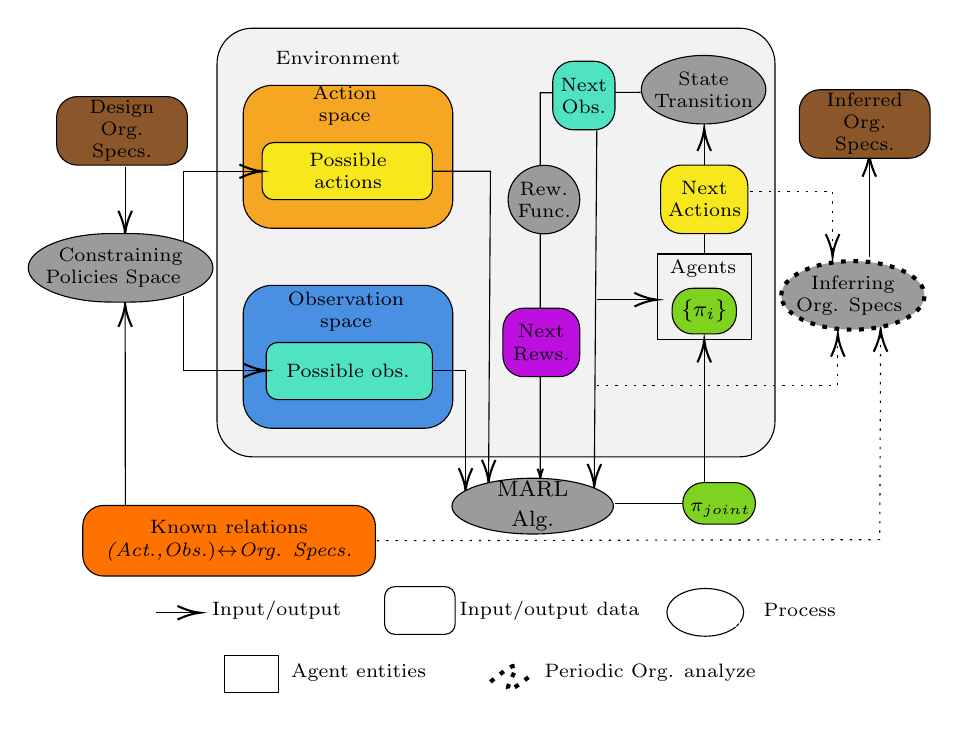
\begin{tikzpicture}[x=0.75pt,y=0.75pt,yscale=-1,xscale=1]
%uncomment if require: \path (0,1124); %set diagram left start at 0, and has height of 1124

%Shape: Rectangle [id:dp9937795244635512] 
\draw  [fill={rgb, 255:red, 242; green, 242; blue, 242 }  ,fill opacity=1 ] (108.97,721) .. controls (108.97,711.61) and (116.58,704) .. (125.97,704) -- (360.78,704) .. controls (370.17,704) and (377.78,711.61) .. (377.78,721) -- (377.78,893.49) .. controls (377.78,902.88) and (370.17,910.49) .. (360.78,910.49) -- (125.97,910.49) .. controls (116.58,910.49) and (108.97,902.88) .. (108.97,893.49) -- cycle ;
%Straight Lines [id:da6518751125509914] 
\draw    (335.62,932.92) -- (300.7,932.92) ;
%Straight Lines [id:da34207082497735786] 
\draw    (313,734.86) -- (264.7,735.09) -- (264.7,918.61) ;
\draw [shift={(264.7,920.61)}, rotate = 270] [color={rgb, 255:red, 0; green, 0; blue, 0 }  ][line width=0.75]    (4.37,-1.32) .. controls (2.78,-0.56) and (1.32,-0.12) .. (0,0) .. controls (1.32,0.12) and (2.78,0.56) .. (4.37,1.32)   ;
%Straight Lines [id:da9417034389402881] 
\draw    (343.7,754.18) -- (343.7,812.75) ;
\draw [shift={(343.7,752.18)}, rotate = 90] [color={rgb, 255:red, 0; green, 0; blue, 0 }  ][line width=0.75]    (10.93,-3.29) .. controls (6.95,-1.4) and (3.31,-0.3) .. (0,0) .. controls (3.31,0.3) and (6.95,1.4) .. (10.93,3.29)   ;
%Straight Lines [id:da4463435210078386] 
\draw    (343.7,922.88) -- (343.7,856.05) ;
\draw [shift={(343.7,854.05)}, rotate = 90] [color={rgb, 255:red, 0; green, 0; blue, 0 }  ][line width=0.75]    (10.93,-3.29) .. controls (6.95,-1.4) and (3.31,-0.3) .. (0,0) .. controls (3.31,0.3) and (6.95,1.4) .. (10.93,3.29)   ;
%Straight Lines [id:da8247669117759437] 
\draw    (291.96,834.78) -- (300.52,834.78) -- (318.99,834.78) ;
\draw [shift={(320.99,834.78)}, rotate = 180] [color={rgb, 255:red, 0; green, 0; blue, 0 }  ][line width=0.75]    (10.93,-3.29) .. controls (6.95,-1.4) and (3.31,-0.3) .. (0,0) .. controls (3.31,0.3) and (6.95,1.4) .. (10.93,3.29)   ;
%Rounded Rect [id:dp13052707912371297] 
\draw  [fill={rgb, 255:red, 245; green, 166; blue, 35 }  ,fill opacity=1 ] (121.59,745.3) .. controls (121.59,737.7) and (127.75,731.53) .. (135.35,731.53) -- (208.78,731.53) .. controls (216.39,731.53) and (222.55,737.7) .. (222.55,745.3) -- (222.55,786.6) .. controls (222.55,794.2) and (216.39,800.36) .. (208.78,800.36) -- (135.35,800.36) .. controls (127.75,800.36) and (121.59,794.2) .. (121.59,786.6) -- cycle ;
%Rounded Rect [id:dp7026077814365836] 
\draw  [fill={rgb, 255:red, 74; green, 144; blue, 226 }  ,fill opacity=1 ] (121.59,841.66) .. controls (121.59,834.06) and (127.75,827.89) .. (135.35,827.89) -- (208.78,827.89) .. controls (216.39,827.89) and (222.55,834.06) .. (222.55,841.66) -- (222.55,882.96) .. controls (222.55,890.56) and (216.39,896.72) .. (208.78,896.72) -- (135.35,896.72) .. controls (127.75,896.72) and (121.59,890.56) .. (121.59,882.96) -- cycle ;
%Rounded Rect [id:dp7429651229296941] 
\draw  [fill={rgb, 255:red, 248; green, 231; blue, 28 }  ,fill opacity=1 ] (130.7,764.57) .. controls (130.7,761.53) and (133.17,759.06) .. (136.21,759.06) -- (207.2,759.06) .. controls (210.24,759.06) and (212.7,761.53) .. (212.7,764.57) -- (212.7,781.09) .. controls (212.7,784.13) and (210.24,786.6) .. (207.2,786.6) -- (136.21,786.6) .. controls (133.17,786.6) and (130.7,784.13) .. (130.7,781.09) -- cycle ;
%Rounded Rect [id:dp2626666197665244] 
\draw  [fill={rgb, 255:red, 80; green, 227; blue, 194 }  ,fill opacity=1 ] (132.7,860.9) .. controls (132.7,857.86) and (135.17,855.39) .. (138.21,855.39) -- (207.2,855.39) .. controls (210.24,855.39) and (212.7,857.86) .. (212.7,860.9) -- (212.7,877.42) .. controls (212.7,880.46) and (210.24,882.92) .. (207.2,882.92) -- (138.21,882.92) .. controls (135.17,882.92) and (132.7,880.46) .. (132.7,877.42) -- cycle ;
%Straight Lines [id:da37906510942957117] 
\draw    (291.96,750.8) -- (290.72,922.92) ;
\draw [shift={(290.7,924.92)}, rotate = 270.41] [color={rgb, 255:red, 0; green, 0; blue, 0 }  ][line width=0.75]    (10.93,-3.29) .. controls (6.95,-1.4) and (3.31,-0.3) .. (0,0) .. controls (3.31,0.3) and (6.95,1.4) .. (10.93,3.29)   ;
%Straight Lines [id:da8878827995944159] 
\draw  [dash pattern={on 0.84pt off 2.51pt}]  (361.37,782.47) -- (405.54,782.47) -- (405.54,812.13) ;
\draw [shift={(405.54,814.13)}, rotate = 270] [color={rgb, 255:red, 0; green, 0; blue, 0 }  ][line width=0.75]    (10.93,-3.29) .. controls (6.95,-1.4) and (3.31,-0.3) .. (0,0) .. controls (3.31,0.3) and (6.95,1.4) .. (10.93,3.29)   ;
%Straight Lines [id:da8073435187842593] 
\draw  [dash pattern={on 0.84pt off 2.51pt}]  (291.96,876.08) -- (408.07,876.08) -- (408.07,853.3) ;
\draw [shift={(408.07,851.3)}, rotate = 90] [color={rgb, 255:red, 0; green, 0; blue, 0 }  ][line width=0.75]    (10.93,-3.29) .. controls (6.95,-1.4) and (3.31,-0.3) .. (0,0) .. controls (3.31,0.3) and (6.95,1.4) .. (10.93,3.29)   ;
%Straight Lines [id:da9521506867066192] 
\draw    (137.99,947.66) -- (64.8,947.66) -- (64.7,838.92) ;
\draw [shift={(64.7,836.92)}, rotate = 89.95] [color={rgb, 255:red, 0; green, 0; blue, 0 }  ][line width=0.75]    (10.93,-3.29) .. controls (6.95,-1.4) and (3.31,-0.3) .. (0,0) .. controls (3.31,0.3) and (6.95,1.4) .. (10.93,3.29)   ;
%Straight Lines [id:da8173351196218479] 
\draw  [dash pattern={on 0.84pt off 2.51pt}]  (177.06,950.92) -- (428.26,950.41) -- (428.69,850.92) ;
\draw [shift={(428.7,848.92)}, rotate = 90.25] [color={rgb, 255:red, 0; green, 0; blue, 0 }  ][line width=0.75]    (10.93,-3.29) .. controls (6.95,-1.4) and (3.31,-0.3) .. (0,0) .. controls (3.31,0.3) and (6.95,1.4) .. (10.93,3.29)   ;
%Straight Lines [id:da6053298376683525] 
\draw    (64.7,770.92) -- (64.7,800.92) ;
\draw [shift={(64.7,802.92)}, rotate = 270] [color={rgb, 255:red, 0; green, 0; blue, 0 }  ][line width=0.75]    (10.93,-3.29) .. controls (6.95,-1.4) and (3.31,-0.3) .. (0,0) .. controls (3.31,0.3) and (6.95,1.4) .. (10.93,3.29)   ;
%Straight Lines [id:da8641416537329594] 
\draw    (423.21,814.13) -- (423.21,766.57) ;
\draw [shift={(423.21,764.57)}, rotate = 90] [color={rgb, 255:red, 0; green, 0; blue, 0 }  ][line width=0.75]    (10.93,-3.29) .. controls (6.95,-1.4) and (3.31,-0.3) .. (0,0) .. controls (3.31,0.3) and (6.95,1.4) .. (10.93,3.29)   ;
%Shape: Rectangle [id:dp009612592743657444] 
\draw   (320.99,812.75) -- (366.42,812.75) -- (366.42,854.05) -- (320.99,854.05) -- cycle ;
%Shape: Boxed Line [id:dp9105440631185389] 
\draw    (79.7,985.61) -- (98.84,985.61) ;
\draw [shift={(100.84,985.61)}, rotate = 180] [color={rgb, 255:red, 0; green, 0; blue, 0 }  ][line width=0.75]    (10.93,-3.29) .. controls (6.95,-1.4) and (3.31,-0.3) .. (0,0) .. controls (3.31,0.3) and (6.95,1.4) .. (10.93,3.29)   ;
%Shape: Rectangle [id:dp18940852352890292] 
\draw   (112.7,1006.17) -- (138.7,1006.17) -- (138.7,1023.94) -- (112.7,1023.94) -- cycle ;
%Curve Lines [id:da6070406744312455] 
\draw [line width=1.5]  [dash pattern={on 1.69pt off 2.76pt}]  (240.7,1018.92) .. controls (271.17,993.71) and (230.78,1040.06) .. (261.24,1014.84) ;
%Straight Lines [id:da04181106466856366] 
\draw    (92.7,806.92) -- (92.7,772.92) -- (128.7,772.92) ;
\draw [shift={(130.7,772.92)}, rotate = 180] [color={rgb, 255:red, 0; green, 0; blue, 0 }  ][line width=0.75]    (10.93,-3.29) .. controls (6.95,-1.4) and (3.31,-0.3) .. (0,0) .. controls (3.31,0.3) and (6.95,1.4) .. (10.93,3.29)   ;
%Straight Lines [id:da5269327271789521] 
\draw    (92.7,832.92) -- (92.7,868.92) -- (130.7,868.92) ;
\draw [shift={(132.7,868.92)}, rotate = 180] [color={rgb, 255:red, 0; green, 0; blue, 0 }  ][line width=0.75]    (10.93,-3.29) .. controls (6.95,-1.4) and (3.31,-0.3) .. (0,0) .. controls (3.31,0.3) and (6.95,1.4) .. (10.93,3.29)   ;
%Straight Lines [id:da8384029096649059] 
\draw    (228.7,924.92) -- (228.7,868.92) -- (212.7,868.92) ;
\draw [shift={(228.7,926.92)}, rotate = 270] [color={rgb, 255:red, 0; green, 0; blue, 0 }  ][line width=0.75]    (10.93,-3.29) .. controls (6.95,-1.4) and (3.31,-0.3) .. (0,0) .. controls (3.31,0.3) and (6.95,1.4) .. (10.93,3.29)   ;
%Straight Lines [id:da8549749304566603] 
\draw    (212.7,772.92) -- (240.7,772.92) -- (239.8,920.92) ;
\draw [shift={(239.79,922.92)}, rotate = 270.35] [color={rgb, 255:red, 0; green, 0; blue, 0 }  ][line width=0.75]    (10.93,-3.29) .. controls (6.95,-1.4) and (3.31,-0.3) .. (0,0) .. controls (3.31,0.3) and (6.95,1.4) .. (10.93,3.29)   ;

% Text Node
\draw (177.2,1014.42) node  [font=\small] [align=left] {{\scriptsize Agent entities}};
% Text Node
\draw (317.7,1014.42) node  [font=\small] [align=left] {{\scriptsize Periodic Org. analyze}};
% Text Node
\draw    (189.7,978.02) .. controls (189.7,975.26) and (191.94,973.02) .. (194.7,973.02) -- (218.7,973.02) .. controls (221.46,973.02) and (223.7,975.26) .. (223.7,978.02) -- (223.7,991.02) .. controls (223.7,993.78) and (221.46,996.02) .. (218.7,996.02) -- (194.7,996.02) .. controls (191.94,996.02) and (189.7,993.78) .. (189.7,991.02) -- cycle  ;
\draw (206.7,984.52) node  [font=\small] [align=left] {\begin{minipage}[lt]{20.08pt}\setlength\topsep{0pt}
\begin{center}
\textcolor[rgb]{1,1,1}{{\tiny assaaaa}}
\end{center}

\end{minipage}};
% Text Node
\draw (269.2,984.42) node  [font=\small] [align=left] {{\scriptsize Input/output data}};
% Text Node
\draw (137.7,984.42) node  [font=\small] [align=left] {{\scriptsize Input/output}};
% Text Node
\draw    (325.7,985.42) .. controls (325.7,979.07) and (333.98,973.92) .. (344.2,973.92) .. controls (354.42,973.92) and (362.7,979.07) .. (362.7,985.42) .. controls (362.7,991.77) and (354.42,996.92) .. (344.2,996.92) .. controls (333.98,996.92) and (325.7,991.77) .. (325.7,985.42) -- cycle  ;
\draw (344.2,985.42) node  [font=\small] [align=left] {\begin{minipage}[lt]{22.12pt}\setlength\topsep{0pt}
\begin{center}
\textcolor[rgb]{1,1,1}{{\tiny aassssaa}}
\end{center}

\end{minipage}};
% Text Node
\draw (389.7,984.42) node  [font=\small] [align=left] {{\scriptsize Process}};
% Text Node
\draw  [fill={rgb, 255:red, 139; green, 87; blue, 42 }  ,fill opacity=1 ]  (31.7,746.92) .. controls (31.7,741.4) and (36.18,736.92) .. (41.7,736.92) -- (84.7,736.92) .. controls (90.22,736.92) and (94.7,741.4) .. (94.7,746.92) -- (94.7,759.92) .. controls (94.7,765.45) and (90.22,769.92) .. (84.7,769.92) -- (41.7,769.92) .. controls (36.18,769.92) and (31.7,765.45) .. (31.7,759.92) -- cycle  ;
\draw (63.2,753.42) node  [font=\scriptsize] [align=left] {\begin{minipage}[lt]{40.43pt}\setlength\topsep{0pt}
\begin{center}
Design\\Org. Specs.
\end{center}

\end{minipage}};
% Text Node
\draw  [fill={rgb, 255:red, 155; green, 155; blue, 155 }  ,fill opacity=1 ]  (249.21,786.55) .. controls (249.21,777.43) and (256.94,770.05) .. (266.46,770.05) .. controls (275.99,770.05) and (283.72,777.43) .. (283.72,786.55) .. controls (283.72,795.66) and (275.99,803.05) .. (266.46,803.05) .. controls (256.94,803.05) and (249.21,795.66) .. (249.21,786.55) -- cycle  ;
\draw (266.46,786.55) node  [font=\scriptsize,xslant=-0.02] [align=left] {\begin{minipage}[lt]{20.58pt}\setlength\topsep{0pt}
\begin{center}
Rew.\\Func.
\end{center}

\end{minipage}};
% Text Node
\draw (165.76,716.05) node  [font=\scriptsize] [align=left] {\begin{minipage}[lt]{42.81pt}\setlength\topsep{0pt}
\begin{center}
Environment
\end{center}

\end{minipage}};
% Text Node
\draw (170.49,741.51) node  [font=\scriptsize] [align=left] {\begin{minipage}[lt]{43.61pt}\setlength\topsep{0pt}
\begin{center}
Action space
\end{center}

\end{minipage}};
% Text Node
\draw (171.12,840.63) node  [font=\scriptsize] [align=left] {\begin{minipage}[lt]{62.26pt}\setlength\topsep{0pt}
\begin{center}
Observation space
\end{center}

\end{minipage}};
% Text Node
\draw (172.07,772.83) node  [font=\scriptsize] [align=left] {\begin{minipage}[lt]{54.32pt}\setlength\topsep{0pt}
\begin{center}
Possible actions
\end{center}

\end{minipage}};
% Text Node
\draw (172.07,869.19) node  [font=\scriptsize] [align=left] {\begin{minipage}[lt]{45.19pt}\setlength\topsep{0pt}
\begin{center}
Possible obs.
\end{center}

\end{minipage}};
% Text Node
\draw  [fill={rgb, 255:red, 155; green, 155; blue, 155 }  ,fill opacity=1 ]  (261.04, 934.24) circle [x radius= 38.89, y radius= 13.44]   ;
\draw (261.04,934.24) node  [font=\small] [align=left] {\begin{minipage}[lt]{37.13pt}\setlength\topsep{0pt}
\begin{center}
{\footnotesize MARL Alg.}
\end{center}

\end{minipage}};
% Text Node
\draw  [fill={rgb, 255:red, 126; green, 211; blue, 33 }  ,fill opacity=1 ]  (333.36,932.92) .. controls (333.36,927.4) and (337.84,922.92) .. (343.36,922.92) -- (358.36,922.92) .. controls (363.88,922.92) and (368.36,927.4) .. (368.36,932.92) .. controls (368.36,938.45) and (363.88,942.92) .. (358.36,942.92) -- (343.36,942.92) .. controls (337.84,942.92) and (333.36,938.45) .. (333.36,932.92) -- cycle  ;
\draw (350.86,932.92) node  [font=\scriptsize] [align=left] {\begin{minipage}[lt]{20.95pt}\setlength\topsep{0pt}
\begin{center}
$\displaystyle \pi _{joint}$
\end{center}

\end{minipage}};
% Text Node
\draw  [fill={rgb, 255:red, 155; green, 155; blue, 155 }  ,fill opacity=1 ]  (313.39,733.6) .. controls (313.39,724.48) and (326.82,717.1) .. (343.39,717.1) .. controls (359.96,717.1) and (373.39,724.48) .. (373.39,733.6) .. controls (373.39,742.71) and (359.96,750.1) .. (343.39,750.1) .. controls (326.82,750.1) and (313.39,742.71) .. (313.39,733.6) -- cycle  ;
\draw (343.39,733.6) node  [font=\scriptsize] [align=left] {\begin{minipage}[lt]{37.77pt}\setlength\topsep{0pt}
\begin{center}
State\\Transition \ 
\end{center}

\end{minipage}};
% Text Node
\draw  [fill={rgb, 255:red, 189; green, 16; blue, 224 }  ,fill opacity=1 ]  (246.7,848.88) .. controls (246.7,843.35) and (251.18,838.88) .. (256.7,838.88) -- (273.7,838.88) .. controls (279.22,838.88) and (283.7,843.35) .. (283.7,848.88) -- (283.7,861.88) .. controls (283.7,867.4) and (279.22,871.88) .. (273.7,871.88) -- (256.7,871.88) .. controls (251.18,871.88) and (246.7,867.4) .. (246.7,861.88) -- cycle  ;
\draw (265.2,855.38) node  [font=\scriptsize] [align=left] {\begin{minipage}[lt]{22.57pt}\setlength\topsep{0pt}
\begin{center}
Next\\Rews.
\end{center}

\end{minipage}};
% Text Node
\draw  [fill={rgb, 255:red, 255; green, 114; blue, 0 }  ,fill opacity=1 ]  (44.27,943.92) .. controls (44.27,938.4) and (48.75,933.92) .. (54.27,933.92) -- (175.27,933.92) .. controls (180.79,933.92) and (185.27,938.4) .. (185.27,943.92) -- (185.27,957.92) .. controls (185.27,963.45) and (180.79,967.92) .. (175.27,967.92) -- (54.27,967.92) .. controls (48.75,967.92) and (44.27,963.45) .. (44.27,957.92) -- cycle  ;
\draw (114.77,950.92) node  [font=\scriptsize] [align=left] {\begin{minipage}[lt]{93.15pt}\setlength\topsep{0pt}
\begin{center}
Known relations\\\textit{(Act.,Obs.})$\displaystyle \leftrightarrow $\textit{Org. Specs.}
\end{center}

\end{minipage}};
% Text Node
\draw  [fill={rgb, 255:red, 155; green, 155; blue, 155 }  ,fill opacity=1 ]  (18,819.42) .. controls (18,810.31) and (35.91,802.92) .. (58,802.92) -- (67,802.92) .. controls (89.09,802.92) and (107,810.31) .. (107,819.42) .. controls (107,828.54) and (89.09,835.92) .. (67,835.92) -- (58,835.92) .. controls (35.91,835.92) and (18,828.54) .. (18,819.42) -- cycle  ;
\draw (62.5,819.42) node  [font=\scriptsize] [align=left] {\begin{minipage}[lt]{57.49pt}\setlength\topsep{0pt}
\begin{center}
Constraining\\Policies Space \ \ \ 
\end{center}

\end{minipage}};
% Text Node
\draw  [fill={rgb, 255:red, 80; green, 227; blue, 194 }  ,fill opacity=1 ]  (270.7,729.92) .. controls (270.7,724.4) and (275.18,719.92) .. (280.7,719.92) -- (290.7,719.92) .. controls (296.22,719.92) and (300.7,724.4) .. (300.7,729.92) -- (300.7,742.92) .. controls (300.7,748.45) and (296.22,752.92) .. (290.7,752.92) -- (280.7,752.92) .. controls (275.18,752.92) and (270.7,748.45) .. (270.7,742.92) -- cycle  ;
\draw (285.7,736.42) node  [font=\scriptsize] [align=left] {\begin{minipage}[lt]{17.81pt}\setlength\topsep{0pt}
\begin{center}
Next\\Obs.
\end{center}

\end{minipage}};
% Text Node
\draw (343.14,819.98) node  [font=\scriptsize] [align=left] {\begin{minipage}[lt]{24.96pt}\setlength\topsep{0pt}
\begin{center}
Agents
\end{center}

\end{minipage}};
% Text Node
\draw  [fill={rgb, 255:red, 126; green, 211; blue, 33 }  ,fill opacity=1 ]  (328.2,839.28) .. controls (328.2,833.76) and (332.68,829.28) .. (338.2,829.28) -- (349.2,829.28) .. controls (354.73,829.28) and (359.2,833.76) .. (359.2,839.28) -- (359.2,841.28) .. controls (359.2,846.81) and (354.73,851.28) .. (349.2,851.28) -- (338.2,851.28) .. controls (332.68,851.28) and (328.2,846.81) .. (328.2,841.28) -- cycle  ;
\draw (343.7,840.28) node  [font=\footnotesize] [align=left] {\begin{minipage}[lt]{18.45pt}\setlength\topsep{0pt}
\begin{center}
$\displaystyle \{\pi _{i}\}$
\end{center}

\end{minipage}};
% Text Node
\draw  [fill={rgb, 255:red, 248; green, 231; blue, 28 }  ,fill opacity=1 ]  (322.7,779.92) .. controls (322.7,774.4) and (327.18,769.92) .. (332.7,769.92) -- (354.7,769.92) .. controls (360.22,769.92) and (364.7,774.4) .. (364.7,779.92) -- (364.7,792.92) .. controls (364.7,798.45) and (360.22,802.92) .. (354.7,802.92) -- (332.7,802.92) .. controls (327.18,802.92) and (322.7,798.45) .. (322.7,792.92) -- cycle  ;
\draw (343.7,786.42) node  [font=\scriptsize] [align=left] {\begin{minipage}[lt]{26.14pt}\setlength\topsep{0pt}
\begin{center}
Next\\Actions
\end{center}

\end{minipage}};
% Text Node
\draw  [color={rgb, 255:red, 0; green, 0; blue, 0 }  ,draw opacity=1 ][fill={rgb, 255:red, 155; green, 155; blue, 155 }  ,fill opacity=1 ][dash pattern={on 1.69pt off 2.76pt}][line width=1.5]   (380.82,832.71) .. controls (380.82,823.6) and (396.27,816.21) .. (415.32,816.21) .. controls (434.38,816.21) and (449.82,823.6) .. (449.82,832.71) .. controls (449.82,841.82) and (434.38,849.21) .. (415.32,849.21) .. controls (396.27,849.21) and (380.82,841.82) .. (380.82,832.71) -- cycle  ;
\draw (415.32,832.71) node  [font=\scriptsize] [align=left] {\begin{minipage}[lt]{44.39pt}\setlength\topsep{0pt}
\begin{center}
Inferring\\Org. Specs \ \ 
\end{center}

\end{minipage}};
% Text Node
\draw  [fill={rgb, 255:red, 139; green, 87; blue, 42 }  ,fill opacity=1 ]  (389.5,743.62) .. controls (389.5,738.09) and (393.98,733.62) .. (399.5,733.62) -- (442.5,733.62) .. controls (448.02,733.62) and (452.5,738.09) .. (452.5,743.62) -- (452.5,756.62) .. controls (452.5,762.14) and (448.02,766.62) .. (442.5,766.62) -- (399.5,766.62) .. controls (393.98,766.62) and (389.5,762.14) .. (389.5,756.62) -- cycle  ;
\draw (421,750.12) node  [font=\scriptsize] [align=left] {\begin{minipage}[lt]{40.43pt}\setlength\topsep{0pt}
\begin{center}
Inferred\\Org. Specs.
\end{center}

\end{minipage}};


\end{tikzpicture}
    \caption{A summary view of the PRAHOM process}
    \label{fig:prahom_process}
\end{figure}

% \RestyleAlgo{ruled}
% \SetKwComment{Comment}{// }{}

% \begin{algorithm}[hbt!]
%     \caption{Partial Relations with Agent History and Organization Model (PRAHOM)}\label{alg:prahom}

%     \KwData{$d$, the Dec-POMDP to solve}
%     \KwData{$ep_{max} \in \mathbb{N}$, the maximum number of episodes}
%     \KwData{$step_{max} \in \mathbb{N}$, the maximum number of steps per episodes}
%     \KwData{$s \in \mathbb{R}$, the cumulative reward expectancy}
%     \KwData{$\pi_{joint}$, the joint-policies to be trained}
%     \KwData{$os_{init}$, the design specifications to respect}
%     \KwData{$Solv$, a MARL algorithm updating policies to solve a Dec-POMDP}

%     \KwResult{$(s\pi_{joint,s,i} \in S\Pi_{joint,s,i}, os_{s,i} \in OS_{s,i})$, the sub-optimal policies associated organization specifications}

%     $s\pi_{joint,s,i} = PRAHOM-sop-training(s,i)$

%     $os_{s,i} = PRAHOM-pos(s\pi_{joint,s,i})$

% \end{algorithm}

\paragraph{\textbf{Inferring Organizational Specifications}}

Rather than using joint-policies directly, we use the joint-histories since they may be built with observed resulting actions when observations are received during a series of test episodes. Indeed, for a given policy $\pi \in \Pi$, the associated history is by definition $h \in h_{joint} = \langle(\omega_k,a_k) | k \in \mathbb{N}\rangle$ and the $(\omega_k,a_k) \in \pi$.
Then, due to the difficulty of inferring information related to organizational specifications, it is possible to associate each observation or action with organization specifications as a \textquote{many to many} relation. It sets up a first frame for identifying organizational specifications in histories. We address that problem in the remainder of this section.

One can define some relations between $\mathcal{M}OISE^+$ specifications and joint-histories. Their premises come from noticing some specifications in the $\mathcal{M}OISE^+$ organizational model can be mapped to subsets of actions from a single suboptimal joint-policy.
From these relations, it is possible to use empirical or statistical approaches to infer organizational specifications out of joint-histories. Below we informally describe key points for understanding that process.

As we have only one group, we do not consider the inter-links and inter-compatibilities. Additionally, as a simplification, we consider only one social scheme.
First, we look at the individual level by trying to figure out the roles, links, sub-groups, individual goals, missions, and plans played by agents by sampling history subsequences $h \in H$ and comparing with known history subsequences whose we know the associated role via the established relations.

After analyzing several joint-policies, we try to reinforce a global view of the goals, missions, plans, and the knowledge of the mission to the goal; with the partially inferred information at the individual level.
In the end, our process tries to synthesize the knowledge inferred until having a better view of the agent cardinality per sub-group, the agent cardinality for each mission, the role cardinality, the compatibilities between roles, the permissions, and obligations.

\paragraph{\textbf{Constraining Policies Space}}

We consider a given MARL algorithm that iteratively converges towards a joint-policy so that each agent's policy is updated at each step until a finite horizon.
We favored the Proximal Policy Optimization for its proven effectiveness in cooperative multi-agent environments without the need for domain-specific algorithmic modifications or architectures~\cite{Yu2022}.
To constrain the possible joint-policies to the ones satisfying the design organizational specifications $os_{init}$, we propose to constrain the action and observation sets for each agent according to $os_{init}$  at each step. For instance, we may constrain an agent to converge to a given role by forbidding actions related to other roles. We used that idea, to set up our process to guide the training according to some design organizational constraints.

First, we use the previously established relations between organizational specifications and action-observation couples, to determine the authorized or forbidden actions playable by agents at each step.
Then, it first computes the authorized actions set $A_{step}$ according to the current history $h_{joint,i}$. Then, an action is chosen among authorized actions. That action $a_{step} \in A_{step}$ is added in history to be used for updating the agent's policy in the next step. Then, the MARL algorithm updates the joint-policy hence the agents' policies with the current action and observation.
Finally, an analysis of the current suboptimal joint-policy $\pi_{joint}$ satisfying $os_{init}$ is triggered periodically. It enables iteratively improving the efficiency of joint-policies and the accuracy of the inferred organizational specifications.
We can note the restriction implied by $os_{init}$ in the possible joint-policies might prevent the MARL algorithm from finding a joint-policy that satisfies the minimal expected cumulative reward defined by the designer.

\subsection{Engineering tool}

PettingZoo is a library that offers a standardized API that simplifies the development of environments with agents and facilitates the application of MARL algorithms.
We developed \emph{PRAHOM PettingZoo Wrapper}\label{PettingZoo-wrapper}, a tool to help automate the setting up of \emph{PRAHOM} for a given PettingZoo environment.
It is a Proof of Concept that enables linking actions with $\mathcal{M}OISE^+$ specifications and defining the organizational specifications. It provides functions to extract the resulting suboptimal raw organizational specifications. During training, actions are masked to guide an agent to learn to act according to the organizational specifications.

\begin{lstlisting}[language=Python, caption=PRAHOM PettingZoo Wrapper basic use, label={lst:wrapper_basic_use}]
from omarl_experiments import PrahomWrapper
env = PettingZoo_env.parallel_env(render_mode="human")
...
action_to_specs = {"agent_name": {
        "14": "role='leader';link='(agent_0,agent_1,auth);..."
        ...}    
    ...}
training_specs = {
    "leadadversary_0": {
        "must": ["(23,41)"],
        "must_not": ["(14,74)"]}...}
env = PrahomWrapper(env, action_to_specs, training_specs, unknown_specs_inference=True, pca_output=True)
# ...TRAINING...
env.prahom_render_pca()
trained_specs, agent_to_specs = env.prahom_specs()
\end{lstlisting}

In \autoref{lst:wrapper_basic_use}, we detailed a basic use of the wrapper to augment a PettingZoo environment (l. 12) with known relations between actions and organizational specifications (l. 4) and the design constraints agents are to satisfy (l. 8). After training, we can print a Principal Component Analysis (PCA) of each agent history over an episode (l.14) which is an additional analysis tool to manually detect emerging roles. It also provides the inferred $\mathcal{M}OISE^+$ specifications considering the last episodes and how agents are instantiated in the last episode.

These results are constructed via empirical or statistical approaches using provided known relations between observations, actions, and organizational specifications. When no relation is available, it tries to detect subsequences of joint-histories likely to match an organizational specification (l. 12). Due to these limitations, the results may not fully describe the underlying organization or may contain noisy inferred organizational specifications. Since the results are compliant with $\mathcal{M}OISE^+$, it is then possible to use them with available MAS design methods to benefit from the identified emerging organizational specifications during the design process.

% We start defining actions with known specifications Focusing of the "lead adversary", we have:

% "observations": [self_vel, self_pos, landmark_rel_positions, other_agent_rel_positions, other_agent_velocities, leader_comm]
% "actions": [say_0, say_1, say_2, say_3] X [no_action, move_left, move_right, move_down, move_up]

% =============

% \subsection{Premises for AOMEA's theoretical core}

% - Organizational oriented MARL: a general research study focusing in integrating the organization in MARL at several aspects
% - DMO (Dec-POMDP MOISE+ OMARL): a class of algorithm falling into OMARL purposes that use MOISE+ as organizational model and Dec-POMDP as a MARL model
% - PRAHOM (Partial Relations with Agent History and Organization Model): a DMO algorithm that allows both getting the organizational specifications out of trained agents; and driving their training to satisfy extra design organizational specifications as constraints.

% \subsection{AOMEA for engineering}

% - We proposed PRAHOM (Partial Relations with Agent History and Organization Model): an algorithm that allows both getting the organizational specifications out of trained agents; and driving their training to satisfy extra design organizational specifications as constraints.
% - [Algo PRAHOM...]

% - We developped PRAHOM as a PettingZoo-wrapper to help in applying the proposed MAS design approach...
% - [Lien vers dépôt GitHub]
% - Description des fonctionalités

% - The general approach workflow follows:
% 1) Reproducing target environment in simulation
% 2) Defining the reward function so agents aim to achieve the goals
% 3) Adding agents to be trained to solve the previously defined problem
% 4) Launching the training in simulation with PRAHOM
% 5) Getting the raw organizational specifications with PRAHOM
% 6) Curating these to produce a safe MAS model
% 7) Using that model to implement a proper MAS
% 8) Check viability and requirements respect in simulation
% 9) Deploy that MAS in the target system

% \begin{itemize}
%     \item Questions at the Multi-Agent System level (system-centric approach)
%           \begin{itemize}
%               \item Number of agents, what heterogeneity?
%               \item What is the common medium (Environment) shared by the agents?
%               \item What communication mechanisms are available to agents?
%               \item What are the communication languages, ontologies, interaction protocols used by the agents?
%               \item What is the organization within which the agents operate? How is it established?
%               \item How do the agents coordinate their actions? How to ensure coherent operation?
%           \end{itemize}

%     \item Agent level questions (agent-centered approach)
%           \begin{itemize}
%               \item What does an agent represent? What actions should be encapsulated in an agent?
%               \item How do agents represent the environment and organization in which they operate?
%               \item How do agents handle interactions with other agents?
%               \item What is the internal structure of the agents?
%           \end{itemize}
% \end{itemize}

% ====================================================================================================

\section{Evaluation in cooperative game environments}

% Evaluation
%     In order to verify and demonstrate the approach, is applied on the following case study.
% 	Case study


In order to assess AOMEA, we considered using \emph{PRAHOM} in available simulated environments made up of agents that have to achieve a goal with the best performance through various collective strategies whose some can be easily understood (presented in \autoref{fig:simulated_environments}).
We selected three Atari-like environments for their visual rendering is a convenient way to assess the results with manual observations\footnotemark[1].
We also considered a Cyberdefense environment as a first attempt to apply \emph{PRAHOM} in a non-visual Cyberdefense environment:

\footnotetext[1]{Additional explanation and the examples discussed using \emph{PRAHOM PettingZoo wrapper} are available at \url{https://github.com/julien6/omarl_experiments?tab=readme-ov-file\#tutorial-predator-prey-with-communication}}

\vspace{0.2cm}

% Left column for text
\hspace{-0.6cm}
\begin{minipage}[t]{0.61\textwidth}

    \begin{itemize}
        \item \textquote{Drone swarm - 3rd CAGE Challenge}~\cite{cage_challenge_3_announcement} (CYB) consists of cyberdender agents deployed on networked drones trying to fight against maliciously deployed malware programs. We may expect agents to \allowbreak collectively isolate compromised drones;
        \item \textquote{Pistonball} (PBL)~\cite{Terry2021} consists of a series of pistons to bring a ball from right to left side hence requiring neighbors' representation;
        \item \textquote{Predator-prey with communication}~\cite{Lowe2017} (PPY) consists of predators monitored by a leader to better catch faster prey hence requiring collective hunting strategies;
        \item \textquote{Knights Archers Zombies}~\cite{Terry2021} (KAZ) consists in a few knights and archers learning how to kill as many zombies hence requiring efficient agent spatial positioning.
    \end{itemize}

\end{minipage}%
\hfill % Ajoute une marge horizontale
% Right column for a figure
\begin{minipage}[t]{0.35\textwidth}
    \vspace{-1cm}
    \begin{figure}[H] % Use the 'H' specifier from the 'float' package to force the figure placement
        \centering
        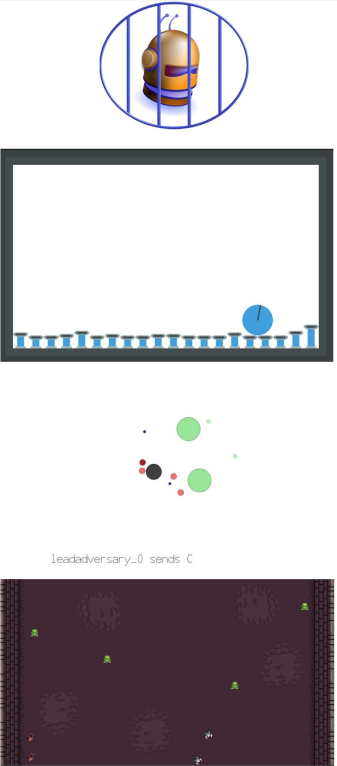
\includegraphics[width=0.6\linewidth]{figures/envs.png} % Replace "example-image" with your figure file name
        \caption{Overview of the selected environments: CYB, PBL, PPY, and KAZ}
        \label{fig:simulated_environments}
    \end{figure}
\end{minipage}

\

\noindent We applied AOMEA in three cases:
\begin{itemize}
    \item No organizational specifications (NTS): agents have to learn the most efficient collective strategies without any constraints or indications.
    \item Partially constraining organizational specifications (PTS): some constraints or indications are given to help converge faster or meet requirements.
    \item Fully constraining organizational specifications (FTS): manually crafted joint-policies are given for they are a reference regarding learned joint-policies.
\end{itemize}

Here, we do not present the details of the constraints that were given in NTS and FTS (available in Git repository\footnotemark[1]).

\begin{figure}[h!]
    \centering
    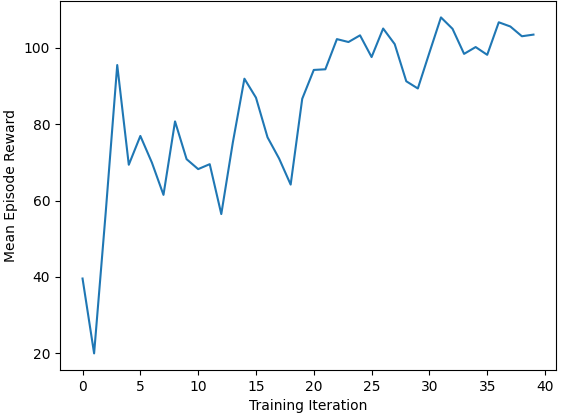
\includegraphics[width=0.8\textwidth]{figures/prahom_learning_curve.png}
    \caption{Average reward for each iteration in the PBL environment for the NTS, PTS, and FTS cases}
    \label{fig:prahom_learning_curve}
\end{figure}

\begin{figure}[h!]
    \centering
    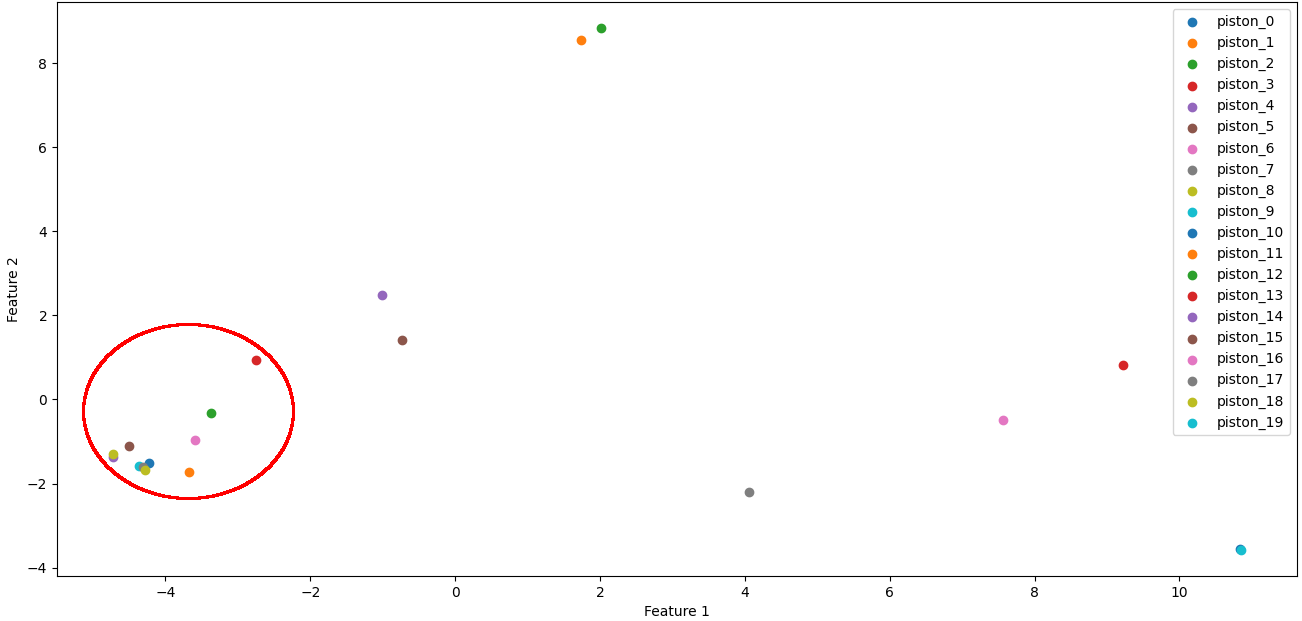
\includegraphics[width=0.8\textwidth]{figures/prahom_pca_analysis.png}
    \caption{PCA of the trained agents' histories in the PBL environment}
    \label{fig:prahom_pca_analysis}
\end{figure}

We evaluate the impact of \emph{PRAHOM} on the following criteria: convergence time ratios between PTS, NTS, and FTS for reaching a threshold cumulative reward. Performance stability shows how the trained agents can achieve the goal generally by assessing several environments generated with different parameters. Results are presented in Table~\ref{tab:training_AOMEA_results}.
%
\begin{table}[t!]

    \centering

    \begin{tblr}{colspec={llll},rows={m},measure=vbox,stretch=-1}

        \textbf{Environment} & \textbf{PTS/NTS} & \textbf{PTS/FTS} & \textbf{Perf. stability \\ (avg. / max)} \\

        \hline

        { PPL }
        & { 4.7 }
        & { 1.3 }
        & { 0.9 } \\

        \hline[dashed]

        { PPY }
        & { 6.3 }
        & { 2.2 }
        & { 0.78 } \\

        \hline[dashed]

        { KAZ }
        & { 4.0 }
        & { 1.1 }
        & { 0.42 } \\

        \hline[dashed]

        { CYB }
        & { 12 }
        & { 3.3 }
        & { 0.36 } \\


    \end{tblr}

    \caption{View of the AOMEA approach impact during training}

    \label{tab:training_AOMEA_results}

\end{table}

%
As a general observation, we can notice convergence time is longer for NTS than for PTS which is also longer than for FTS. As expected, the search space is decreasing, hence a shorter convergence time. For instance, we noticed a faster convergence to a sub-optimal solution in the PBL environment by providing organizational specifications as presented in \autoref{fig:prahom_learning_curve}. Although PTS converges faster than NTS to a comparable cumulative reward, NTS may outperform PTS because trained agents' policies are hand-tailored to solve the problem much more finely than the designer's organizational specifications can do. Low-performance stability in the more complex CYB environment indicates that the trained agents have difficulty finding general strategies compared to the agents in the other environments.

We also took into account the following criteria after training: roles, links, and global performance. A qualitative analysis is presented in Table~\ref{tab:trained_AOMEA_results}
%
\begin{table}[t!]

    \centering

    \begin{tblr}{colspec={llll},rows={m},measure=vbox,stretch=-1}

        \textbf{Environment} & \textbf{Roles} & \textbf{Links} & \textbf{Global performance} \\

        \hline

        { 1 }
        & {  }
        & {  } \\
        & {  } \\

        \hline[dashed]

        { 2 }
        & {  }
        & {  } \\
        & {  } \\

        \hline[dashed]

        { 3 }
        & {  }
        & {  } \\
        & {  } \\

        \hline[dashed]

        { 4 }
        & {  }
        & {  } \\
        & {  } \\

        \hline[dashed]

        { 5 }
        & {  }
        & {  } \\
        & {  } \\

    \end{tblr}

    \caption{View of the OOMARL approach impact after training}

    \label{tab:trained_OOMARL_results}

\end{table}

%
% //TODO: Moise+ schemes and comparison with expected ones
%
For the PBL environment, we can notice roles being equivalent for agents are expected to act the same. Indeed, trained agents' histories are close hence showing a common emerging role. We generate the PCA presented in \autoref{fig:prahom_pca_analysis} by expressing agents' histories as vectors containing the observation-action couples. We can notice most agents’ histories are in the left bottom zone (circled in red). It shows most pistons seem to act similarly as expected. We observe no organizational specifications except roles have been generated because agents cannot communicate. For the KAZ environment, we can notice two distinct roles: archers tend to move away from zombies, while knights tend to approach them. For the PPY environment, we can observe the output specifications indicate authority links between the leader predator and the simple predators to enable collective strategies for circling prey. Finally, the CYB environment shows communications between blue agents are indeed understood as communication links that enable isolating infiltrated drones or trying to fix and alert recently suspected drones.

For the CYB environment, we developed our custom MAS via a simple hand-crafted decision tree as preconized in AOMEA in light of the organizational specifications we curated by removing noisy results. Our approach did not suggest general roles but relevant strategy patterns have been identified. For instance, regarding links between agents' roles, we noticed that the agents sending messages frequently seem to be spotted as suspected by their neighbors. In addition, a cyber-defender agent in the communication radius of a suspected drone tends to switch off its communication and reactivate afterward. Even though these insights are few, the mean score we got with our curated MAS is about -2000 which is indeed close to the top 5 scores. This shows AOMEA to be indeed applicable to the Cyberdefense context additionally bringing safety guarantees.

\section{Conclusion}

% =======> demande toi avant de rédiger la conclusion "Qu'est ce qui change dans l'état de l'art avec ce papier ?"... si tu avais lu ce papier et qu'il n'était pas de toi qu'est ce que tu te serai dis 

%  - Need for easing the MAS design by assisting human designer
%  - We proposed a novel general MAS design approach that consists in getting relevant organizational specifications out of agents in training satisfying design constraints. These insights allow implementing a suited safe MAS to be deployed on target system
%  - We validated that approach for various different environments including in a Cyberdefense context.
%  - Main perspective is to improve the reliability of PRAHOM between organizational specifications and agents' training satisfying to design constraints.
%  - Another future work is to reduce the manual parts of our approach with implementation of a full integrated development environment.

% 1er paragraphe: résumé + qu'est-ce qui est changé par rapport à l'edt
% 2ème paragraphe: perspectives et future works

% In this article we presented AOMEA, a novel general MAS design approach that aims to ease the MAS designing when it can not be easily conducted by designers in highly complex deployment environments.
MAS methodological works rely on the designer's knowledge to design a suited MAS organization but do not provide automatic or assisted ways to determine relevant organizational mechanisms.
%solely from the design requirements and the global goal.
MARL techniques have been successfully applied to train agents automatically to reach the given goal without explicit characterization of emergent collective strategies.
AOMEA's originality is to augment a MARL process with an explicit organizational model towards a methodological purpose to address these issues. We first exposed how AOMEA is intended to be used in MAS engineering as an additional tool to assist in the design process.
Then, we explained the AOMEA's theoretical core with links between Dec-POMDP and the $\mathcal{M}OISE^+$ through the \emph{PRAHOM} process.
Furthermore, we implemented the \emph{PRAHOM PettingZoo wrapper} as a Proof of Concept for practically applying AOMEA and we showed it enables getting some organizational specifications that satisfy the design constraints and allow achieving the given goal.
Finally, we applied our approach in four PettingZoo environments to assess the impact on and after training. The obtained performance results show to be comparable to known ones showing our approach to be viable.

Even though \emph{PRAHOM} is agnostic of the MARL algorithm because it uses agents' histories to infer organizational specifications, reconstructing agents' collective behaviors a posteriori may be difficult. Indeed, a major perspective for improving \emph{PRAHOM} is to go further with supervised and non-supervised learning techniques in addition to empirical statistical approaches for identifying valuable organizational specifications from joint-histories. Moreover, it is worth investigating recent works in MARL techniques such as hierarchical learning because they already seek to characterize emergent strategies throughout learning.
%Eventually, we also aim to improve AOMEA applicability by developing dedicated interfaces built around \emph{PRAHOM} making it more accessible for industrial and research contexts.


% ---- Bibliography ----
%
% BibTeX users should specify bibliography style 'splncs04'.
% References will then be sorted and formatted in the correct style.
%
% \bibliographystyle{splncs04}
% \bibliography{mybibliography}
%
\section*{References}

% \bibliographystyle{abbrv}
\bibliographystyle{splncs04}

\bibliography{references}

\end{document}